\documentclass[10pt,a4paper,twoside]{book}
\usepackage[utf8]{inputenc}
\usepackage{amsmath}
\usepackage{amsfonts}
\usepackage{amssymb}
\usepackage{graphicx}
\usepackage{hyperref}
\usepackage{subcaption}
\usepackage{minted}
\usepackage[left=2.5cm,right=2.5cm,top=3.5cm,bottom=3cm]{geometry}
\usepackage{algorithm}
\usepackage{algpseudocode}
\usepackage{placeins}
\newtheorem{mydef}{Theorem}
\DeclareMathOperator*{\argmax}{arg\,max}
\DeclareMathOperator*{\argmin}{arg\,min}
\newtheorem{defini}{Definition}



\makeindex

\begin{document}
\title{Bayesian optimization in machine learning}
\author{Jos\'e Jim\'enez Luna}
\maketitle
\tableofcontents


\chapter{Organization of this work}

\section{Introduction}

This Master's Thesis provides an introduction to both Gaussian Processes and Bayesian Optimization. This work aims to be a multi-objective optimization task:

\begin{itemize}
\item The first objective of the thesis is to provide the reader with an introduction to Gaussian Process regression and Bayesian optimization. The work is written in such a way that it alternates very often between theoretical and practical (in terms of programming) background. This master's thesis resembles a programming book or a manual. All the examples seen through this work were coded from scratch.
\item To show the Bayesian Optimization framework works in several real-world machine learning tasks. I do so by selecting several datasets (most of them from medical, biological or physical phenomena), applying such methodology and comparing to other common strategies applied for the same problem. 
\item Finally, to write a complete software package for users to apply Bayesian Optimization in their research. This comes in the form of a Python ($>$3.5) package named pyGPGO. The code can be accessed through \url{https://github.com/hawk31/pyGPGO}. The entire software package is MIT licensed. All the examples and code snippets throughout this manual are based on this software. While certainly there are a couple implementations of Global Optimization software in Python, the software described here is modular, very minimalistic and requires minimal dependencies, while still maintaining most of the other's functionality
\end{itemize}

We begin by describing the title of this thesis. Bayesian Optimization focuses on the global optimization of a function $f:\mathbb{R}^n \rightarrow \mathbb{R}$ over a compact set $A$. The problem can be formalized as:

\begin{equation}
\max_{\boldsymbol{x}\in A} f(x)
\end{equation}

Most optimization procedures (local based ones such as gradient ascent, for example) assume that the function $f$ is closed-form, that is, it has an analytical expression, that it is convex, with known first or second order derivatives or cheap to evaluate. Bayesian optimization focuses on all these problems proposing a very elegant solution. By the use of a surrogate model, a Gaussian Process, a Bayesian optimization procedure can help find the global minimum of non-necessarily convex, expensive functions that are expensive to evaluate. These methods shine also where there is no closed-form expression to evaluate and does not need any function derivatives.\\

Now is when the machine learning part of the title comes into play. In machine learning (also known as statistical learning), we are usually interested in minimizing a loss function $\mathcal{L}$. These losses can take many forms. For instance, when doing regression, a typical loss might be the mean squared error between predictions and observed values on a holdout test set.

\begin{equation}
\mathcal{L}(\boldsymbol{y}, \boldsymbol{\hat{y}}) = \dfrac{1}{n} \sum_i \left(y_i - \hat{y_i}\right)^2
\end{equation}

In binary classification, for example, a very popular choice is the logarithmic loss:

\begin{equation}
\mathcal{L}(\boldsymbol{y}, \boldsymbol{\hat{y}}) = -\dfrac{1}{n} = \sum_i \left(y_i \log(\hat{y_i}) + (1 - y_i)\log(1-\hat{y_i})\right)
\end{equation}

Notice in any case, that these losses are typically defined in a subset of $\mathbb{R}$. We focus on the supervised setting of machine learning, and more specifically regression. Depending on the problem at hand, even evaluating these losses can be very expensive from a computational point of view. This may have to do with the machine learning algorithm used or the size of the dataset at hand. These machine learning algorithms typically have \textit{hyperparameters}, that is, parameters that have to be tuned in a sensible way to get the best performance possible out of these models. In the machine learning community it is common for practitioners to do an hyperparameter grid search or even randomize it. Since the training of a single model can already take substantial resources in terms of CPU cycles or memory, we would like to have a more efficient and cheap way to optimize these hyperparameters. Bayesian optimization will let us do that by proposing the next candidate point $\boldsymbol{x}$ to evaluate according to several criteria.

\section{Organization of the thesis}

Before we dive directly into the topic at hand, it is mandatory to explain how this manual is intended to be read. Different chapters will cover different material, so if the reader is familiar with a topic in a chapter, for example, the chapter on Gaussian Processes, he can skip directly to the chapter on Bayesian Optimization or to the implementation if he wishes. \\

\textbf{Chapter 2} focuses on a swift but thorough introduction to regression problems using Gaussian Processes. These are the surrogate models we will use for Bayesian Optimization in Chapter 3. We will cover the theory behind them both from a weight space point of view and from a functional point of view. We will also explain different covariance functions and their role in these models, as well as methods for optimizing their hyperparameters. Finally we will provide the reader with usable code to fit a Gaussian Process in a regression problem. This chapter is heavily based on Carl E. Rasmussen excellent book \textit{Gaussian Processes for Machine Learning}[ref], an more specially in chapters 2, 4 and 5. In fact, if the reader is interested in a more advanced, wider, slowly-paced introduction to Gaussian Processes, this is by far the best resource to go to. \\

\textbf{Chapter 3} is about the main topic in this work, Bayesian Optimization. Once we have laid down all the foundations of Gaussian Processes, we can start explaining the theory of Bayesian optimization using these as surrogate models. The algorithms, while simple, are very powerful. The role of several acquisition functions, that is to say, the functions that will propose the next point to evaluate will be discussed, as well as their advantages or disadvantages. The references on this chapter will be more diverse than on the previous chapter, as I will try to summarize several publications. Readers already familiar with Gaussian Processes should jump directly into this chapter.\\

\textbf{Chapter 4} covers experiments using the software provided alongside this manual. These are mostly mid-sized regression or classification problems where we will compare the performance of Bayesian Optimization of hyperparameters with several regressors/classifiers with other strategies, such as random search or simulated annealing. Most of these datasets are related to experimental sciences, and some of them were used for other benchmarking purposes in other studies. \\

\textbf{Chapter 5} has no theoretical content nor testing content. It will cover technical explanations of pyGPGO, the software developed alongside this manual. Software usage examples are also provided. 

\chapter{Gaussian Process regression}

 In this chapter we will focus on regression problems. Assume we have some labelled data $D = \left\lbrace \left(\boldsymbol{x_i}, y_i\right) | i = 1,\dots,n\right\rbrace$, where $\boldsymbol{x}$ is a vector of covariates and $y$ denotes a continuous objective variable. We wish to learn a predictive distribution over new values of $\boldsymbol{x}$, so that we can make predictions and inference over these. In practice, for simplicity we write that $D = \left(X, \boldsymbol{y}\right)$, where $X$ is our predictor matrix.\\

One can interpret a Gaussian Process in several ways. The most widely known is the function space view, which is the one we will cover first here and the one we will assume for the rest for the thesis. In this view, we consider a Gaussian Process to be a stochastic process, hence, a distribution over functions, instead of over values. Inference takes place directly in this space. For completeness, we will also provide a weight-space view second, that might be more appealing to readers familiar with Bayesian linear regression.\\



\section{A function space view for Gaussian Processes}

We start by formally defining a Gaussian Process:

\begin{defini}
A Gaussian Process as a collection of random variables, any finite number of which have a joint Gaussian distribution. This process is totally defined by two functions. Its \textit{mean function}:

\begin{equation}
m(\boldsymbol{x}) = \mathbb{E}\left[f(\boldsymbol{x})\right]
\end{equation} 

and its \textit{covariance function}:

\begin{equation}
k(\boldsymbol{x}, \boldsymbol{x'}) = \mathbb{E}\left[\left( f(\boldsymbol{x}) - m(\boldsymbol{x}) \right)\left( f(\boldsymbol{x}') - m(\boldsymbol{x}')\right)\right]
\end{equation}


We say that $f$ is a Gaussian Process with mean $m(\boldsymbol{x})$ and covariance function $k(x, x')$ and write:

\begin{equation}
f(\boldsymbol{x}) \sim \mathrm{GP}\left(m(\boldsymbol{x}), k(\boldsymbol{x}, \boldsymbol{x'}) \right)
\end{equation}
\end{defini}

In practice, for simplicity we will take $m(\boldsymbol{x}) = 0$, but this can be specified otherwise. As stated before, a Gaussian Process fulfils the marginalization property, that is to say that if the the GP specifies $(y_1, y_2) \sim N(\boldsymbol{\mu}, \Sigma)$ then this implies that $y_1 \sim N(\mu_1, \Sigma_{11})$. A Gaussian multivariate distribution is just a finite index set of a Gaussian process. 

As seen in the previous section, a Gaussian Process can be viewed as a Bayesian regression model using a particular kernel, that is, the model $f(\boldsymbol{x}) = \phi(\boldsymbol{x})^T \boldsymbol{w}$ with the same prior as in equation \ref{wprior} has mean and covariance functions:

\begin{align}
\mathbb{E}\left[f(\boldsymbol{x})\right] = \phi(\boldsymbol{x})^T\mathbb{E}\left[\boldsymbol{w}\right] = 0\\
\mathbb{E}\left[f(\boldsymbol{x})f(\boldsymbol{x'})\right] = \phi(\boldsymbol{x})^T\mathbb{E}\left[\boldsymbol{w}\boldsymbol{w}^T\right]
\phi(\boldsymbol{x'}) = \phi(\boldsymbol{x})^T\Sigma_p\phi(\boldsymbol{x'})
\end{align}

It is now a good time to start specifying several covariance functions, the \textit{squared exponential} kernel, defined as:

\begin{equation}
k(x, x') = \exp\left(-\dfrac{1}{2}|x - x'|^2\right)
\end{equation}

where $|.|$ denotes the standard $L_2$ norm. Most of the covariance functions that we will see here are a function of this norm, therefore it is much more comfortable to write $r = |x - x'|$ and therefore the squared exponential kernel becomes:

\begin{equation}
\label{sqexp}
k(r) = \exp\left(-\dfrac{1}{2}r^2\right)
\end{equation}

It is straightforward to draw samples from a Gaussian Process. In particular, since we work with a finite number of points, choose an arbitrary number of them $X_*$ and compute the squared exponential kernel. Then the procedure is simplified to just samplimg from the following multivariate Gaussian:

\begin{equation}
\label{fprior}
\boldsymbol{f_*} \sim N\left(\boldsymbol{0}, K(X_*, X_*)\right)
\end{equation}

To illustrate this point, we will write a very simple Python script to draw samples from this function. For the moment, consider evenly spaced samples with a step of $\dfrac{\pi}{16}$. All code produced here and in other examples uses pyGPGO, the developed software alongside this thesis. In particular, the code available in Appendix \ref{drawGP} produces Figure \ref{fig:drawPrior}.\\

\begin{figure}
\caption{Three sampled Gaussian Process priors using the Squared Exponential kernel.}
\label{fig:drawPrior}
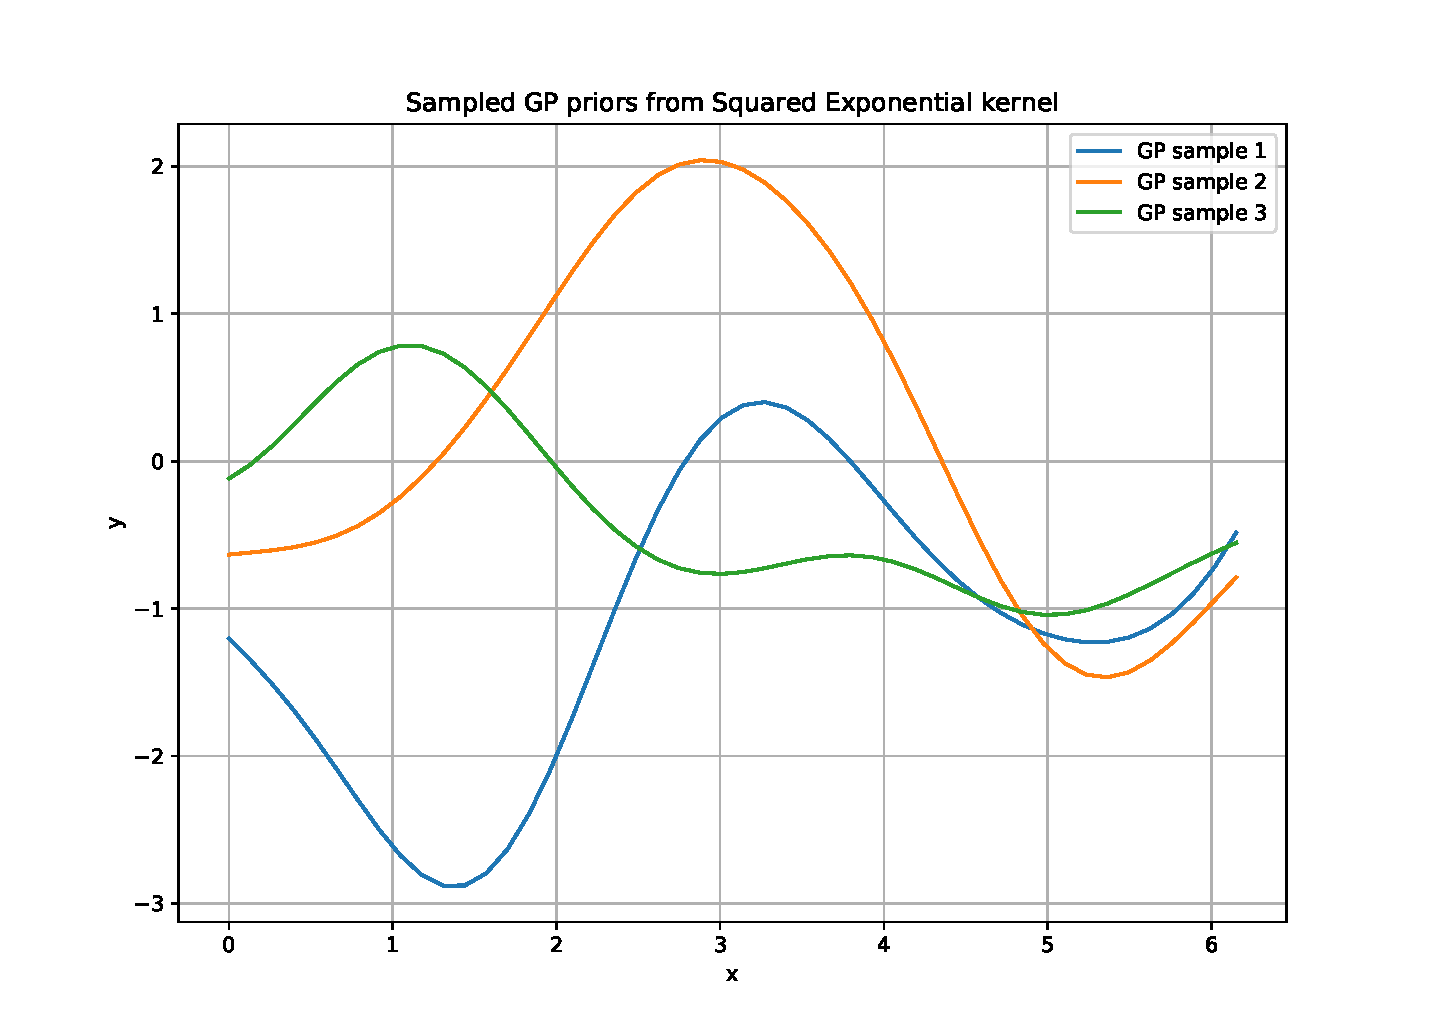
\includegraphics[width=\textwidth]{figures/chapter2/drawPrior}
\end{figure}

There's one important concept to explain before we move on. Notice in Figure \ref{fig:drawPrior} that the drawn functions seem to have a characteristic length-scale. This can be interpreted as the distance you have to move in input space before the function value changes significantly. By default, the squared exponential kernel uses a characteristic length-scale of 1 ($l = 1$). To change this behaviour to another, it is sufficient to consider $r/l$ instead of $r$ in Equation \ref{sqexp}. This can be thought as an hyperparameter to optimize, but we will return to this in another section.

\section{A weight space view for Gaussian Processes}

In this section we will try to draw connections between Bayesian linear regression and  Gaussian Processes, through the use of kernel functions. 

\subsection{Standard Bayesian linear regression}

A Bayesian linear regression model with Gaussian error can be formulated as:

\begin{equation}
\label{linearmodel}
y = X^T \boldsymbol{w} + \epsilon
\end{equation} 

where we typically assume $\epsilon \sim N(0, \sigma_n^2)$. This noise assumption directly implies a Gaussian likelihood, thus it can be easily proven that:

\begin{equation}
p(\boldsymbol{y}|X, \boldsymbol{w}) \sim N (X^T\boldsymbol{w}, \sigma_n^2 I)
\end{equation}

Assume now a Gaussian prior on the weights $\boldsymbol{w}$:

\begin{equation}
\label{wprior}
\boldsymbol{w} \sim N(\boldsymbol{0}, \Sigma_p)
\end{equation}

We are interested now on the posterior distribution of $w$, given both $X$ and $y$, and assuming the model in Equation \ref{linearmodel}, that is:

\begin{equation}
p(\boldsymbol{w}|\boldsymbol{y}, X) = \dfrac{p(\boldsymbol{y}|X, \boldsymbol{w}) p(\boldsymbol{w})}{p(\boldsymbol{y}| X)}
\end{equation}

One can solve this problem by means of sampling procedures like Markov Chain Monte Carlo, but in this particular case, there is a closed-form solution. It can be proven quite easily that:

\begin{equation}
p(\boldsymbol{w}|X, \boldsymbol{y}) \sim N \left(\dfrac{1}{\sigma_n^n}A^{-1}X\boldsymbol{y}, A^{-1}\right)
\end{equation}

where $A = \sigma^{-2}XX^T + \Sigma_p^{-1}$. Notice that a simple MAP (maximum a posteriori) estimate of the weights can be obtained by just computing the mean of this distribution. Now, to make predictions for a particular test case $\boldsymbol{x_{*}}$, we average over all possible parameter values, hence we get a whole predictive distribution. Again, it can be proven that:

\begin{equation}
f_{*}|x_{*}, X, \boldsymbol{y} \sim N\left(\dfrac{1}{\sigma_n^2}\boldsymbol{x_{*}}^T A^{-1}X\boldsymbol{y}, \boldsymbol{x_*}^T A^{-1} \boldsymbol{x}_{*}\right)
\end{equation} 

\subsection{Kernel functions in feature space}

We have presented a very simple Bayesian approach to linear regression in the previous section. While useful, it lacks expressiveness due to its linearity. A very simple idea is to project this data into a higher dimension, where it may be more easily separated by a linear model of this sort. This is called using the kernel trick. We can do this through a covariance (or kernel) function $\phi(\boldsymbol{x})$. Note by $\Phi(X)$ the aggregation of columns after computing this kernel function in the entire dataset at hand.\\

The model becomes now:

\begin{equation}
f(\boldsymbol{x}) = \phi(\boldsymbol{x})^T \boldsymbol{w}
\end{equation}

where we assume the same prior over $\boldsymbol{w}$ as in Equation \ref{wprior}. All the math presented in the previous section applies here, just placing $\phi(\boldsymbol{x})$ instead of $\boldsymbol{x}$. The predictive distribution over $y$ becomes now, for example:

\begin{equation}
\label{torewrite}
f_{*}|x_{*}, X, \boldsymbol{y} \sim N\left( \dfrac{1}{\sigma^2_n}\phi(\boldsymbol{x_*})^T A^{-1}\Phi \boldsymbol{y}, \phi(\boldsymbol{x_*})^T A^{-1}\phi(\boldsymbol{x_*})    \right)
\end{equation}

where for simplicity we have written $\Phi = \Phi(X)$ and $A = \sigma_n^{-2}\Phi\Phi^T + \Sigma_p^{-1}$. The predictive distribution needs to invert $N \times N$ matrix. Equation \ref{torewrite} can be rewritten as:

\begin{equation}
f_{*}|x_{*}, X, \boldsymbol{y} \sim N\left(\boldsymbol{\phi_*}^T\Sigma_p\Phi(K + \sigma^2_n I)^{-1}\boldsymbol{y}, \boldsymbol{\phi_*}\Sigma_p\boldsymbol{\phi_*} - \boldsymbol{\phi_*}^T\Sigma_p\Phi(K + \sigma^2_n I)^{-1}\Phi^T\Sigma_p\boldsymbol{\phi_*}\right)
\end{equation}

where we have again simplified notation by $\boldsymbol{\phi_*} = \phi(\boldsymbol{x_*})$ and $K = \Phi^T\Sigma_p\Phi$. Now notice that the entries of $K$ for both train and test set are of the form  $\phi(\boldsymbol{x_*}^T)\Sigma_p\phi(\boldsymbol{x_*})$. We have implicitly defined now a \textit{covariance function} of the form $k(\boldsymbol{x}, \boldsymbol{x'}) = \phi(\boldsymbol{x_*}^T)\Sigma_p\phi(\boldsymbol{x_*})$. This is in fact an inner product with respect to $\Sigma_p$. That is if we define $\psi(\boldsymbol{x}) = \Sigma_p^{1/2}(\boldsymbol{x})$, then a simple dot product representation of a covariance function is:

\begin{equation}
k(\boldsymbol{x}, \boldsymbol{x'}) = \psi(\boldsymbol{x})^T\psi(\boldsymbol{x'})
\end{equation}

where $\Sigma_p^{1/2}$ can be defined by means of a singular value decomposition. We then replace the original feature vectors by these dot products, \textit{lifting} to a higher space.

\section{Prediction using a Gaussian Process prior}
\label{pred}

In this particular section, arguably the most important one in the chapter, we will learn how to incorporate the knowledge of training data $D = \left\lbrace \left(\boldsymbol{x_i}, y_i\right) | i = 1,\dots,n\right\rbrace$ into our Gaussian Process to obtain a posterior predictive distribution. We will start considering the case that we have a noiseless function, that is to say, when $\sigma^2_n = 0$. Let us define $K(X, X_{*})$, the covariance function evaluated on train and test points, $K(X, X)$ the covariance function evaluated at only the training points, $K(X_{*}, X_{*})$ equivalently defined for the test values. Notice the last two have to be square matrices by definition.\\

Let us also use the following theorem:

\begin{mydef}
\label{conditioning}
Let $\boldsymbol{x}$ and $\boldsymbol{y}$ be jointly Gaussian:
\begin{equation}
\begin{bmatrix}
\boldsymbol{x}\\
\boldsymbol{y}
\end{bmatrix} \sim N\left(
\begin{bmatrix}
\boldsymbol{\mu_x}\\
\boldsymbol{\mu_y}
\end{bmatrix},
\begin{bmatrix}
A   && C \\
C^T && B
\end{bmatrix}
\right)
\end{equation}

Then $\boldsymbol{x|y} \sim \left(\boldsymbol{\mu_x} + C B^{-1}(\boldsymbol{y} - \boldsymbol{\mu_y}), A - CB^{-1}C^T \right)$
\end{mydef}

According to the prior distribution chosen in \ref{fprior}, assume that $\boldsymbol{f}$ and $\boldsymbol{f_*}$ are jointly Gaussian:

\begin{equation}
\begin{bmatrix}
\boldsymbol{f}\\
\boldsymbol{f_*}
\end{bmatrix} \sim N\left(
\boldsymbol{0},
\begin{bmatrix}
K(X, X)  && K(X, X_*) \\
K(X_*, X) && K(X_*, X_*)
\end{bmatrix}
\right)
\end{equation}


We are interested now in the distribution of $\boldsymbol{f_{*}}|\boldsymbol{f}$. Simply applying Theorem \ref{conditioning}, we can obtain:

\begin{equation}
\boldsymbol{f_*|f} \sim N\left(K(X_*, X)K(X, X)^{-1}\boldsymbol{f}, K(X_*, X_*) - K(X_*, X)K(X, X)^{-1}K(X, X_*) \right)
\end{equation}

This covers all the basics for a Gaussian Process regression model. Notice that now we have a complete predictive distribution over test values $\boldsymbol{f_{*}}$, and this provides us with plenty of choices. For example, one could obtain an estimate of this function by drawing samples from a multivariate normal with the computed posterior parameters, or obtain a MAP estimate using the posterior mean.\\

Let us now consider the scenario where observations are not noise-free, that is, each time you query the function there is a i.i.d Gaussian error with mean $0$ and variance $\sigma_n^2 > 0$. Assume now the following prior on the noisy observations:

\begin{equation}
Cov(\boldsymbol{y}) = K(X, X) + \sigma^2_n I 
\end{equation}

Following the exact operations as before, but taking into account this new term, we got the following joint distribution:

\begin{equation}
\begin{bmatrix}
\boldsymbol{f}\\
\boldsymbol{f_*}
\end{bmatrix} \sim N\left(
\boldsymbol{0},
\begin{bmatrix}
K(X, X) + \sigma^2_n I && K(X, X_*) \\
K(X_*, X) && K(X_*, X_*)
\end{bmatrix}
\right)
\end{equation}

And conditioning again $\boldsymbol{f_{*}}$ on $\boldsymbol{f}$, we obtain our final predictive distribution:

\begin{equation}
\boldsymbol{f_*|f} \sim N(\boldsymbol{\overline{f_*}},  Cov(\boldsymbol{f_*}))
\end{equation}

where now:

\begin{align}
\boldsymbol{\overline{f_*}} = K(X_*, X)\left(K(X, X) + \sigma^2_n I   \right)^{-1}\boldsymbol{y}\\
Cov(\boldsymbol{f_*}) = K(X_*, X_*) - K(X_*, X)\left(K(X, X) + \sigma_n^2 I \right)^{-1}K(X, X_*)
\end{align}

It will probably be useful to note that a Gaussian Process model can be written easily in terms of a Bayesian hierarchical model, since:

\begin{align}
\label{hierarchical}
\boldsymbol{y}|\boldsymbol{f} \sim N(\boldsymbol{f}, \sigma^2_n I)\\
\label{hierarchical2}
\boldsymbol{f}|X \sim N(\boldsymbol{0}, K(X, X))
\end{align}

In fact, one can also assume other priors, even over $\sigma_n^2$. This representation may help us understand the introduction of the \textit{marginal likelihood}. This marginal likelihood in a Gaussian Process setting is defined as:

\begin{equation}
p(\boldsymbol{y}|X) = \int p(\boldsymbol{y}|\boldsymbol{f}, X)p(\boldsymbol{f}|X) d\boldsymbol{f}
\end{equation}

Using the results from Equations \ref{hierarchical} and \ref{hierarchical2} we can derive the integral analytically to obtain:

\begin{equation}
\log p(\boldsymbol{y}|X) = - \dfrac{1}{2}\boldsymbol{y}^T(K + \sigma^2_n I)^{-1}\boldsymbol{y} - \dfrac{1}{2}\log |K + \sigma^2_n I| - \dfrac{n}{2}\log 2\pi
\end{equation}

We have now all the necessary ingredients to lay down pseudo-code for your own implementation of a Gaussian Process regressor, as presented in Algorithm \ref{alg}. It makes use of several tricks for computational stability, such as a Cholesky decomposition and several linear system of equations to avoid directly inverting matrices.\\

\begin{algorithm}
	\caption{Gaussian regressor pseudo-code.}
		\label{alg}
		\begin{algorithmic}[1]
			\Function {GPRegressor}{$X$, $\boldsymbol{y}$, $k$, $\sigma_n^2$, $\boldsymbol{x_*}$}
			\State{$L \gets \textrm{chol}(K + \sigma_n^2 I)$}
			\State{$\boldsymbol{\alpha} \gets \textrm{linsolve}\left(L^T, \textrm{linsolve}(L, \boldsymbol{y})\right)$}
			\State{$\overline{f_*} \gets \boldsymbol{k_*}^T\boldsymbol{\alpha}$}
			\State{$\boldsymbol{v} \gets \textrm{linsolve}(L, \boldsymbol{k_*})$}
			\State{$\mathbb{V}\left[f_* \right] \gets k(\boldsymbol{x_*}, \boldsymbol{x_*}) - \boldsymbol{v}^T\boldsymbol{v}$}
			\State{$\log p(\boldsymbol{y}|X) \gets -\dfrac{1}{2}\boldsymbol{y}^T\boldsymbol{\alpha} - \sum_i \log L_{ii} - \dfrac{n}{2}\log 2\pi$}
			\EndFunction
		\end{algorithmic}
\end{algorithm}

pyGPGO includes an implementation of a Gaussian Process regressor under the \texttt{GPRegressor} module. The entire module along with its functionality will be explained in detail in Section \ref{features}.

\subsection{A toy example of Gaussian Process regression}

Now that we have both the algorithm and the tools at hand, it may be interesting how a Gaussian Process regressor behaves with a toy example. We try to approximate a simple sine function in the interval $[0, 2\pi]$, and plot both the posterior mean and a 95\% confidence band using the posterior variance of the fitted process. The code in Appendix \ref{sineGP} produces Figure \ref{fig:GPsine}.\\


\begin{figure}
\caption{A fitted Gaussian Process regressor to samples of the sine function.}
\label{fig:GPsine}
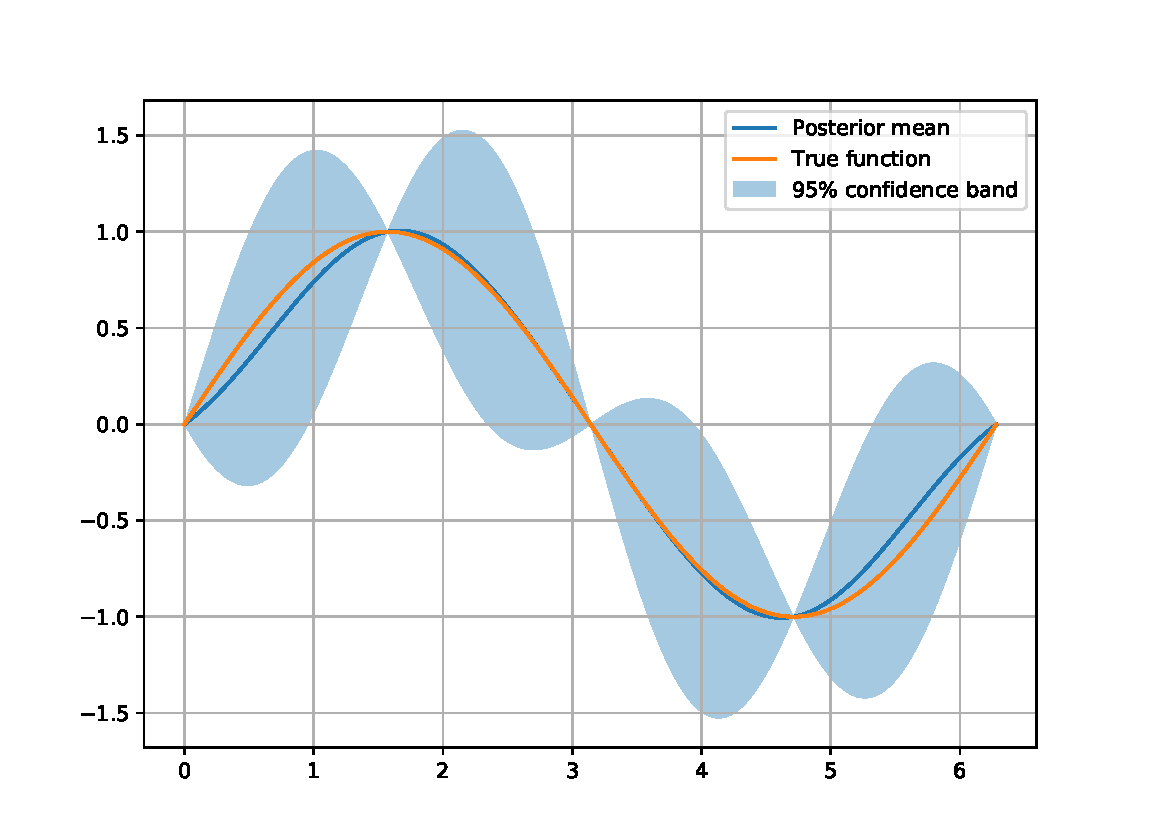
\includegraphics[width=\textwidth]{figures/chapter2/GPsine}
\end{figure}

\subsection{Picking a winner}

In the previous section we have shown how to compute predictive posterior distribution for function outputs $y_*$ given a new input $\boldsymbol{x}_*$. These are given by a Gaussian distribution with a certain mean and variance. In plenty of production settings, however, it is more common to provide a single value, or estimate $y_{\mathrm{guess}}$ that is \textit{optimal} in some sense. To define a sense of optimality, define a loss function $\mathcal{L}(y_{\mathrm{true}}, y_{\mathrm{guess}})$. This, defines a penalty incurred by taking the decision to use $y_{\mathrm{guess}}$ when the true value is $y_{\mathrm{true}}$. For example, this could be the mean square or mean absolute error function. In the Bayesian setting, there is no clear mention of a loss function in any stage. In the frequentist setting, however, a model is usually trained by minimizing this loss. Furthermore, there is a clear separation between loss and likelihood in the Bayesian setting, the latter used for training, with prior information. The loss function however only captures the consequences of making a single specific choice given a true state.\\

Again, we would like to somehow pick a \textit{winner} $y_{\mathrm{guess}}$ that minimizes our loss. Without knowing $y_{\mathrm{true}}$, our best choice is to minimize the expected loss, averaging with respect to our model:

\begin{equation}
\mathcal{R}_{\mathcal{L}}(y_{\mathrm{guess}}|\boldsymbol{x}_*) = \int \mathcal{L}(y_{*}, y_{\mathrm{guess}})p(y_*|\boldsymbol{x}_*, \mathcal{D})dy
\end{equation}

Our optimal value is the one that minimizes this expected loss:

\begin{equation}
\label{risk}
y_{\mathrm{optimal}}|\boldsymbol{x}_* = \argmin_{y_{\mathrm{guess}}}\mathcal{R}_{\mathcal{L}}(y_{\mathrm{guess}}|\boldsymbol{x}_*)
\end{equation}

It can be proven that the value $y_{\mathrm{guess}}$ that minimizes Equation \ref{risk} for the absolute loss function is the median of $p(y_*|\boldsymbol{x}_*,\mathcal{D})$. For the squared loss function, it is the mean of the same distribution. Since in our case we are dealing with the Gaussian distribution, median and mean coincide, and the most reasonable \textit{winner} will therefore be the specific value of the posterior mean. 

\section{On covariance functions}
\label{covariancefunc}

A covariance function, like the squared exponential kernel that we have been using as a example throughout the chapter encodes our assumptions of similarity between inputs from $\boldsymbol{x}$. We assume \textit{similar} items in input space to have similar values of the target value $y$. Not all functions of $\boldsymbol{x}$ and $\boldsymbol{x'}$ can be defined as covariance function. Covariance functions (though not all) tend to satisfy different properties:

\begin{itemize}
\item \textit{Weak stationarity}. A covariance function is said to be weakly stationary if it is a function of $\boldsymbol{x} - \boldsymbol{x'}$. That is to say that it is invariant to translations in the input space. Most of the covariance functions we will see fall into this category.
\item \textit{Isotropy}. A covariance function is said to be isotropic if it is \textit{only} function of  $|\boldsymbol{x} - \boldsymbol{x'}|$. Therefore, every isotropic covariance function is stationary.
\item Dot-product. Some covariance functions are functionals of the dot-product $|\boldsymbol{x}^T \boldsymbol{x'}|$. These kernels, while invariant to rotations are not invariant to translations.
\end{itemize}

There is an excellent theoretical analysis of covariance functions in Chapter 4 of Carl E. Rasmussen's book \textit{Gaussian Processes for Machine Learning}. We will not cover this here since it falls beyond the scope of this thesis. However, we will start providing examples of the most common covariance functions. All covariance functions described here are implemented in the software developed alongside this thesis, pyGPGO, in the \texttt{covfunc} module. We will describe their functionality in Section \ref{features}.\\

The \textit{Squared Exponential} covariance function is the one that we have been using so far. It is also arguably the most used in practice. It takes the general form:

\begin{equation}
k_{SE}(r) = \exp\left(-\dfrac{r^2}{2l^2} \right)
\end{equation}

where $l$ is the parameter controlling its characteristic length-scale. It is useful to define these functions in terms of $r$ since we can abstract this calculation to another function. \\

The \textit{Matern class} of covariance functions takes the form:

\begin{equation}
k_{\textrm{Matern}}(r) = \dfrac{2^{1-\nu}}{\Gamma(\nu)}\left(\dfrac{\sqrt{2\nu} r}{l}    \right)^\nu K_\nu\left( \dfrac{\sqrt{2\nu}r}{l} \right)
\end{equation}

with $\nu, l > 0$ and $K_\nu$ is a modified Bessel function of the second kind.  Simple functional forms can be obtained when $\nu$ is half integer, that is $\nu = p + 1/2$ for $p$ non-negative integer. In particular, if $\nu=1/2$, we obtain the a simple exponential kernel and if we take limit $\nu \rightarrow \infty$ we obtain the squared exponential covariance function. Popular values are $\nu=3/2,\; 5/2$.\\


The $\gamma$-exponential covariance function, of which the squared exponential is a special case. It takes the general form:

\begin{equation}
k(r) = \exp\left( - \left(\dfrac{r}{l}\right)^\gamma  \right)
\end{equation}

for $0 < \gamma \leq 2$. \\

The \textit{Rational Quadratic} covariance function takes the form:

\begin{equation}
k_{RQ}(r) = \left( 1 + \dfrac{r^2}{2\alpha l^2} \right)^{-\alpha}
\end{equation}

with $\alpha, l > 0$. This covariance function can be seen as a scale mixture of squared exponential kernels with different length scales.\\


The \textit{arcSin} kernel is an example of a dot product covariance function, therefore non-stationary:

\begin{equation}
k_{\textrm{arcSin}}(\boldsymbol{x}, \boldsymbol{x'}) = \dfrac{2}{\pi}\sin^{-1}\left(\dfrac{2\boldsymbol{x}\Sigma\boldsymbol{x'}}{\sqrt{(1 + 2\boldsymbol{x}^T\Sigma\boldsymbol{x})(1 + 2\boldsymbol{x'}^T\Sigma\boldsymbol{x})}}   \right)
\end{equation}\\

Normally, these are the covariance functions that are used for the noiseless case of observation, that is, we know precisely that $f(\boldsymbol{x}_i) = y_i, \;\; i=1\dots n$. In general, our covariance functions will take the form:

\begin{equation}
k^y(\boldsymbol{x}_p, \boldsymbol{x}_q) = \sigma^2_f k(\boldsymbol{x}_p, \boldsymbol{x}_q) + \sigma^2_n \delta_{pq} \,
\end{equation}

where $\sigma^2_f$ is the signal variance, and controls the overall scale of our covariance matrix, $\sigma^2_n$ is the noise variance and $\delta_{pq}$ is a Kronecker delta function. Notice we note now $k^y$ instead of $k$ to account for noisy observations. In practice, all covariance function internal parameters plus $\left\lbrace\sigma_n^2, \sigma^2_f\right\rbrace$ can be considered hyperparameters. One can consider them fixed or can try to estimate it from data. We will treat this problem in Section \ref{hyper}.


\subsection{Visualizing different covariance functions}

We have seen plenty of covariance function specifications in the last section. Remember that these control the degree of \textit{similarity} between input points. As an exercise, it would be good to recreate the same sine function example that we saw before, using four different stationary different covariance functions. The choice of parameters is the default one in pyGPGO. The script detailed in Appendix \ref{covzoo} below produces Figure \ref{fig:zoo}. \\


\begin{figure}
\caption{Behaviour of different stationary covariance functions with the default parameters in pyGPGO.}
\label{fig:zoo}
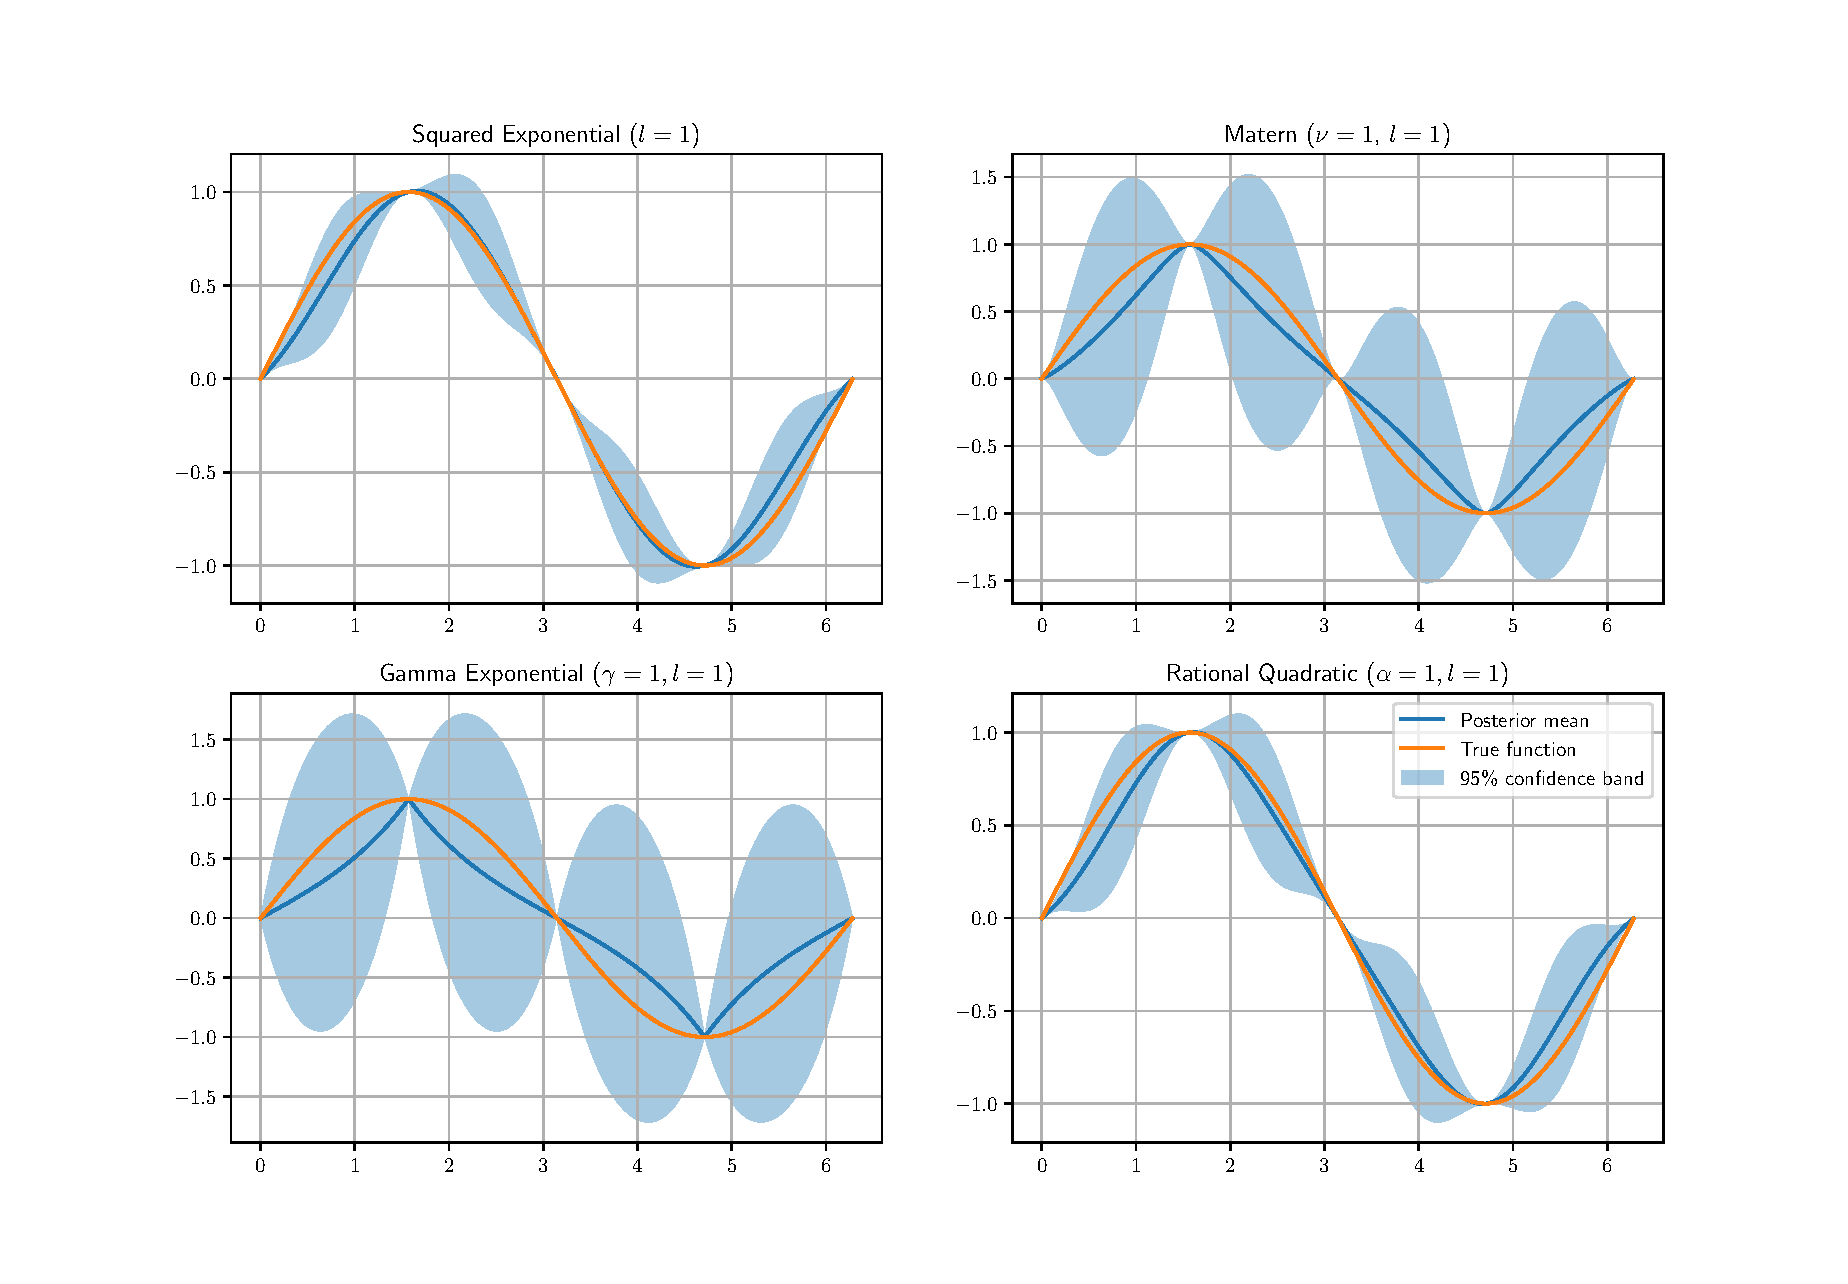
\includegraphics[width=\textwidth]{figures/chapter2/zoo}
\end{figure}

\section{Hyperparameter optimization}
\label{hyper}

As seen in the previous sections, different covariance functions have different \textit{hyperparameters}. These control how the kernel measures similarity among different instances of $\boldsymbol{x}$. So far, we have chosen these hyperparameters according to those set default in pyGPGO, but one may want to optimize these according to the data they have at hand. Depending on the situation, this optimization may lead to better models, either in terms of accuracy or interpretability. There are several ways to select these hyperparameters, one more analytical, by optimizing the marginal log-likelihood, and simpler ones based on cross-validation.

\subsection{Type II Maximum Likelihood}
\label{empbayes}

This is the empirical Bayes analytical approach to optimizing hyperparameters. One may quickly notice that Gaussian Processes are non-parametric models, in the sense that apart from the quantities set in the covariance functions, there is nothing else to optimize for. First we will provide a small background on Bayesian model selection. Assume that we have a model  $\mathcal{H}_i$ with \textit{parameters} $\boldsymbol{w}$, \textit{hyperparameters} $\boldsymbol{\theta}$, and we have some training data $X, \boldsymbol{y}$. The posterior over the parameters is easily given by:

\begin{equation}
\label{posteriorparam}
p(\boldsymbol{w}|\boldsymbol{y}, X, \boldsymbol{\theta}, \mathcal{H}_i) = \dfrac{p(\boldsymbol{y}|X, \boldsymbol{w}, \mathcal{H}_i)p(\boldsymbol{w}|\boldsymbol{\theta}, \mathcal{H}_i)}{p(\boldsymbol{y}|X, \boldsymbol{\theta}, \mathcal{H}_i)}
\end{equation}

where $p(\boldsymbol{y}|X, \boldsymbol{w}, \mathcal{H}_i)$ is the likelihood, $p(\boldsymbol{w}|\boldsymbol{\theta}, \mathcal{H}_i)$ our prior distribution over the parameters and $p(\boldsymbol{y}|X, \boldsymbol{\theta}, \mathcal{H}_i)$ is called the \textit{evidence} or marginal likelihood. Notice that this last quantity is nothing but the integral over parameter $\boldsymbol{w}$ space of the numerator in Equation \ref{posteriorparam}.\\

We can do the same at the next level of inference for the hyperparameters. The posterior of hyperparameters is defined as:

\begin{equation}
\label{posteriorhyper}
p(\boldsymbol{\theta}|\boldsymbol{y}, X, \mathcal{H}_i) = \dfrac{p(\boldsymbol{y}|X, \boldsymbol{\theta}, \mathcal{H}_i)p(\boldsymbol{\theta}|\mathcal{H}_i)}{p(\boldsymbol{y}|X, \mathcal{H}_i)}
\end{equation}

where now $p(\boldsymbol{\theta}|\mathcal{H}_i)$ is our prior over hyperparameters. We are interested however in optimizing the denominator in Equation \ref{posteriorhyper} with respect to the hyperparameters. Typically, in Bayesian inference to perform the kind of integrals presented before, one has to resort to sampling procedures related to Markov Chain Monte Carlo, such as the Gibbs sampler. In the case of Gaussian processes, all computations are analytically tractable. In fact, the expression of the marginal likelihood was presented in Section \ref{pred}. We reproduce the expression here for completeness:

\begin{equation}
\log p(\boldsymbol{y}|X) = - \dfrac{1}{2}\boldsymbol{y}^T(K + \sigma^2_n I)^{-1}\boldsymbol{y} - \dfrac{1}{2}\log |K + \sigma^2_n I| - \dfrac{n}{2}\log 2\pi
\end{equation}

For typical local optimization methods to work fairly well, we may also need an specification of the derivative of the log-marginal likelihood w.r.t. the hyperparameters.

\begin{equation}
\dfrac{\partial}{\partial \theta_j}\log p(\boldsymbol{y}|X, \boldsymbol{\theta}) = \dfrac{1}{2}\boldsymbol{y}^T K^{-1}\dfrac{\partial K}{\partial \theta_j}K^{-1}\boldsymbol{y} - \dfrac{1}{2}\textrm{tr}\left(K^{-1} \dfrac{\partial K}{\partial \theta_j} \right)
\end{equation}

where $\dfrac{\partial K}{\partial \theta_j}$ denotes the derivative of the selected covariance function, evaluated at each pair of instances of the training set. For optimization, one may choose to make use of this expression or not, depending on both of the optimization algorithm (gradient ascent, L-BFGS-B...) or on the cost of evaluation of the derivative. In pyGPGO, most of the covariance functions are implemented with a method \texttt{gradK} to return the gradient. We will come back to detail pyGPGO optimization procedures in Section \ref{features}. 

\subsubsection{Another toy example: Optimizing the characteristic length-scale}

To illustrate the previous point, it may be a good idea to see the behaviour of the marginal log-likelihood and its gradient when we modify the characteristic length scale $l$ in the squared exponential covariance function. The sine function will also serve as playground here. The code in Appendix \ref{hyperopt} produces Figure \ref{fig:logmarginal}.


\begin{figure}
\caption{Log-marginal likelihood and its gradient w.r.t to the characteristic length-scale. Notice there seems to be an optimal point at around $l = 1.4$.}
\label{fig:logmarginal}
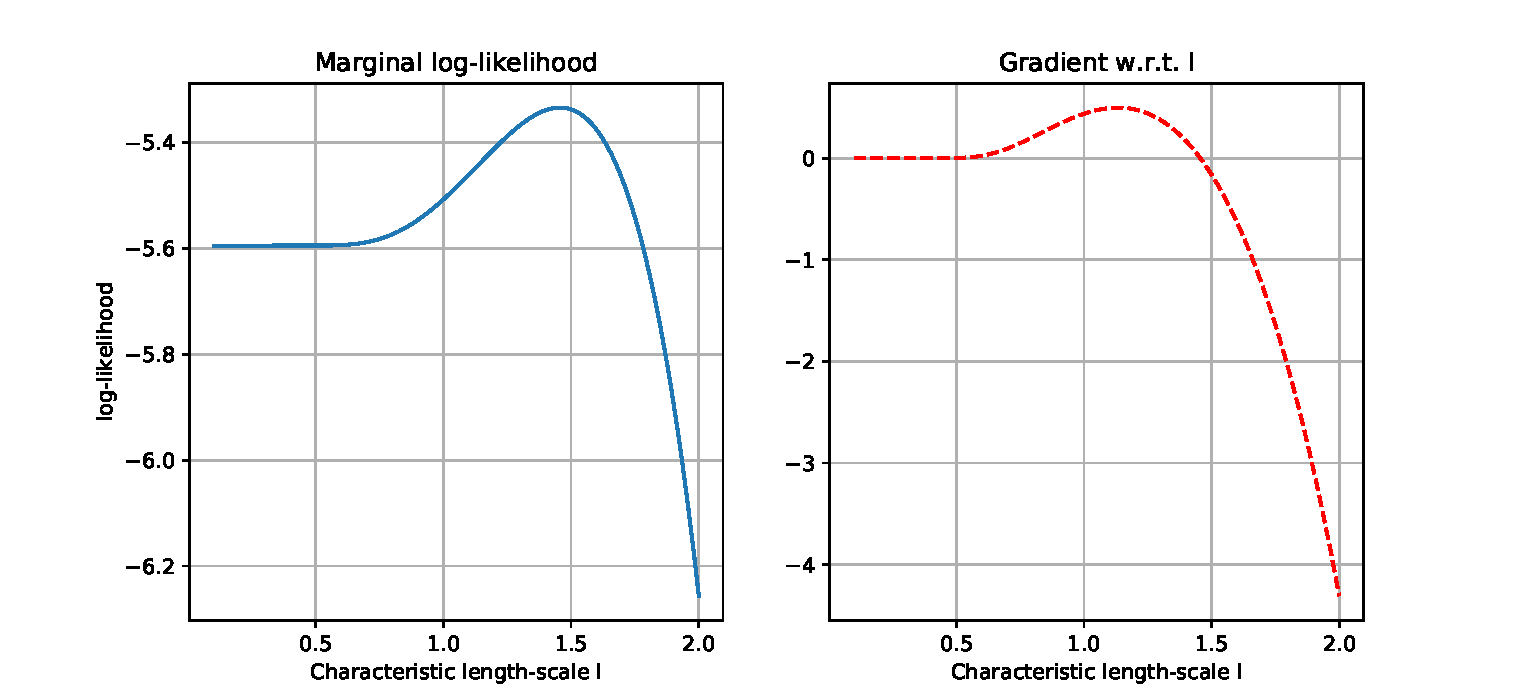
\includegraphics[width=\textwidth]{figures/chapter2/logmarginal}
\end{figure}


\subsection{Cross validation}

There is a very extensive analytical evaluation of cross validation using Gaussian Process in Rasmussen's book. Here, we will only lay down some very basic ideas related to model selection from a very basic machine learning perspective. The concepts presented here are more useful if one plans to use Gaussian Processes only as a regression model, not as a surrogate one towards another objective, as we will do in the following chapter. \\

To evaluate the performance of hyperparameters $\boldsymbol{\theta}$, in $D=\left( X, \boldsymbol{y}\right)$ one could do the following:

\begin{itemize}
\item \textbf{Holdout test}. Consider $D = \left\lbrace D_T, D_V \right\rbrace$ as a training and validation set from your data and $\boldsymbol{\nu}$ the set of hyperparameter vectors $\boldsymbol{\nu}$ to test. Train your Gaussian Process regressor on $D_T$ with some subset of hyperparameters from $\boldsymbol{\nu}$ and test its performance according to some loss metric $\mathcal{L}$ on $D_V$. Choose hyperparameters according to the lower loss obtained.
\item \textbf{$k$-fold cross validation}. Instead of considering a single test set $D_V$, partition $D={D_1,\dots, D_k}$. Train your model iteratively on $k-1$ sets and test on the remaining one. Consider an average of losses for each hyperparameter to test.  
\end{itemize}

\section{Further theoretical aspects}

In this section, we will briefly mention other theoretical aspects of Gaussian Processes. This includes for example, how Gaussian Process can be seen as \textit{linear smoothers}, by means of a spectral analysis or how to incorporate explicit basis functions into the model. Readers can safely skip this section if not particularly interested, as it will not be mentioned any other time throughout the text.

\subsection{Gaussian processes as linear smoothers}

As many machine learning algorithms, the main objective of a Gaussian Process regressor is to reconstruct the underlying signal $f$ by removing noise $\epsilon$. It does this by computing a weighted average of the values $\boldsymbol{y}$. In particular, as seen in \ref{pred}, it can be written as:

\begin{equation}
\overline{f}(\boldsymbol{x}_*) = \boldsymbol{k}(\boldsymbol{x}_*)^T(K + \sigma_n^2 I)^{-1}\boldsymbol{y}
\end{equation}

Therefore, one can see a Gaussian Process regressor as a linear smoother [ref]. We can study this smoothing in terms of spectral analysis [ref]. Again, for training points, predicted training points $\overline{\boldsymbol{f}}$ are:

\begin{equation}
\overline{\boldsymbol{f}} = K(K + \sigma_n^2 I)^{-1}\boldsymbol{y}
\end{equation}

Write $K$ using its eigenvalue decomposition $K = \sum_{i=1}^n \lambda_i \boldsymbol{u}_i\boldsymbol{u}_i^T$, with $\lambda_i$ and $\boldsymbol{u}_i$ its $i$-th eigenvalue and eigenvector respectively. Since $K$ is a covariance matrix, its is symmetric positive semidefinite, and therefore has positive eigenvalues. If we note $\gamma_i = \boldsymbol{u}_i^T\boldsymbol{y}$, then:

\begin{equation}
\overline{\boldsymbol{f}} = \sum_{i=1}^n \dfrac{\gamma_i \lambda_i}{\lambda_i + \sigma^2_n}\boldsymbol{u}_i
\end{equation}

For the covariance functions we have studied in section \ref{covariancefunc}, the eigenvalues are larger for slowly varying eigenvectors, so the more frequent items in $\boldsymbol{y}$ get smoothed-out. The effective number of degrees of freedom in a Gaussian Process model can be defined as the number of used eigenvectors:

\begin{equation}
\mathrm{df}(K) = \mathrm{tr}(K(K + \sigma_n^2 I)^{-1}) = \sum_{i=1}^n\dfrac{\lambda_i}{\lambda_i + \sigma_n^2}
\end{equation}

To make the explanation clearer, let us define $\boldsymbol{h}(\boldsymbol{x}_*) = (K + \sigma_n^2 I)^{-1}\boldsymbol{k}(\boldsymbol{x}_*)$. So for a new given point, prediction is defined as $\overline{f}(\boldsymbol{x}_*)^T \boldsymbol{y}$, that is, a linear combination of $\boldsymbol{y}$, with weights $\boldsymbol{h}(\boldsymbol{x}_*)$. A Gaussian Process regressor is a linear smoother, since the weight function $\boldsymbol{h}$ does not depend directly on $\boldsymbol{y}$. While a regular linear model defines a linear combination of the inputs, a linear smoother defines a linear combination of the targets. This weight function depends directly on the specific location of the $n$ training points, by means of the matrix inversion of $K + \sigma_n^2 I$, therefore observations close in input space are smoothed out.

\subsection{Explicit basis functions}

Notice that during the entire chapter, we have considered a Gaussian Process prior with mean $m(\boldsymbol{x}) = 0$ for simplicity reasons. One may want, however, to define a different mean value for the prior. On the other hand, imposing $m(\boldsymbol{x}) = 0$ is not a strong assumption, since the posterior is not constrained to be zero as well. With an explicit mean function $m(\boldsymbol{x}) \neq 0$, the prior becomes:

\begin{equation}
f(\boldsymbol{x}) \sim \mathcal{G}\mathcal{P}\left(m(\boldsymbol{x}), k(\boldsymbol{x}, \boldsymbol{x^*})\right)
\end{equation}

and the mean of the posterior predictive distribution then becomes, very naturally:

\begin{equation}
\boldsymbol{f}_* = \boldsymbol{m}(X_*) + k(X_*, X)K^{-1}\left(\boldsymbol{y} - \boldsymbol{m}(X)\right) 
\end{equation}

The variance of the posterior predictive distribution remains the same as in Equation \ref{pred}. In practice, however, it may not be clear how to specify a prior mean function for the process. In some cases it may be useful to define a few parametric basis function, whose parameters $\boldsymbol{\beta}$ we have to estimate from training data. Formally:

\begin{equation}
\label{gbasis}
g(\boldsymbol{x}) = f(\boldsymbol{x}) + \boldsymbol{h}(\boldsymbol{x})^T\boldsymbol{\beta}
\end{equation}

where $f(\boldsymbol{x})$ is a regular zero-mean Gaussian Process prior, $\boldsymbol{h}(\boldsymbol{x})$ are our chosen basis functions, and $\beta$ are our parameters. For example, if we are interested in polynomial regression, then $\boldsymbol{h}(x) = (1, x, x^2, \dots)$. One could consider optimizing $\boldsymbol{\beta}$ the same way as with our kernel hyperparameters, but if we assume a Gaussian prior $\boldsymbol{\beta} \sim \mathcal{N}(\boldsymbol{b}, B)$, we can solve analytically to obtain another Gaussian Process:

\begin{equation}
g(\boldsymbol{x}) \sim \mathcal{G}\mathcal{P}\left(\boldsymbol{h}(\boldsymbol{x}^T\boldsymbol{b}, k(\boldsymbol{x}, \boldsymbol{x}^*) + \boldsymbol{h}(\boldsymbol{x})^T B \boldsymbol{h}(\boldsymbol{x}^*)\right)
\end{equation} 

Notice that now we have an extra term in the covariance function. This is caused by the uncertainty in the parameters of the mean. Now predictions are made by substituting these parameters into Equation \ref{gbasis}. An explicit version for the mean and covariance is given by:

\begin{align}
&\overline{\boldsymbol{g}}(X_*) = H^T_* \hat{\boldsymbol{\beta}} + K_*^T K^{-1}(\boldsymbol{y} - H^T\hat{\boldsymbol{\beta}}) = \overline{\boldsymbol{f}}(X_*) + R^T\hat{\boldsymbol{\beta}}\\
&\mathrm{Cov}(\boldsymbol{g_*}) = K_{**} + R^T(B^{-1} + HK^{-1}H^T)^{-1}R
\end{align}

where $H$ and $H_*$ are matrices containing the evaluation of the chosen basis functions over training and testing points respectively, $\hat{\boldsymbol{\beta}} = (B^{-1} + H K^{-1} H^T)^{-1}(H K^{-1}\boldsymbol{y} + B^{-1}\boldsymbol{b})$ and $R = H_* - HK^{-1}K_{*}$. The posterior process parameters can be interpreted as such: $\hat{\boldsymbol{\beta}}$ is a mean of the model linear parameters, a compromise between the prior and the likelihood provided by the data. The mean of the process is simply $\hat{\boldsymbol{\beta}}$ plus our typical Gaussian Process prediction of the residuals. The covariance matrix is just the addition of our regular expression and a non-negative term.\\

Consider the limit of $B^{-1}$ as it approaches $O$ ($O$ being a zero-filled matrix), that is when the prior is vague. We then get a predictive distribution independent of $\boldsymbol{b}$:

\begin{align}
&\overline{\boldsymbol{g}}(X_*) = \overline{\boldsymbol{f}}(X_*) + R^T\hat{\boldsymbol{\beta}}\\
&\mathrm{Cov}(\boldsymbol{g_*}) = K_{**} + R^T\left(HK^{-1}H^T\right)^{-1}R
\end{align}

where now $\hat{\boldsymbol{\beta}} = \left(HK^{-1}H^T\right)^{-1}HK^{-1}\boldsymbol{y}$.\\

We explore now the behaviour of the marginal log-likelihood under this model where we assume a Gaussian prior $\boldsymbol{\beta} \sim \mathrm{N}(\boldsymbol{b}, B)$. Formally:

\begin{equation}
\log p(\boldsymbol{y}|X, \boldsymbol{b}, B) = -\dfrac{1}{2}\log |K + H^T B H| - \dfrac{n}{2}\log 2\pi
\end{equation}

In the same way as before, exploring the limit $B^{-1} \rightarrow O$, the prior becomes irrelevant, so we can safely assume that $\boldsymbol{b} = 0$, yielding:

\begin{align}
\log p(\boldsymbol{y}|X, \boldsymbol{b} =& \boldsymbol{0}, B) = -\dfrac{1}{2}\boldsymbol{y}^T K^{-1}\boldsymbol{y} + \dfrac{1}{2}\boldsymbol{y}^T C \boldsymbol{y}\\
&- \dfrac{1}{2}\left(\log |K| + \log |B| + \log |A| + n\log 2\pi \right)
\end{align}

where $A = B^{-1} + HK^{-1}H^T$ and $C = K^{-1}H^T A^{-1}HK^{-1}$.

\chapter{Bayesian optimization}

\section{Preliminaries}

In this chapter we will deal with the main topic of this master's thesis, Bayesian Optimization. Here, we approach global optimization from the viewpoint of Bayesian theory, as a sequential problem. For the moment, imagine that we have a very expensive function to evaluate $f:\mathbb{R}^n: \rightarrow \mathbb{R}$. This function, for the purposes of this work, will be the negative of a loss function in a machine learning problem, or any other fitness function that we wish to maximize. Formally, we wish to maximize over a compact set $\mathcal{A}$.

\begin{equation}
\max_{\boldsymbol{x}\in \mathcal{A}} f(\boldsymbol{x})
\end{equation}

For technical reasons, we also assume that the function is \textit{Lipschitz-continuous}, that is, there exists some constant $C$ such that $\forall \boldsymbol{x}_1, \boldsymbol{x}_2 \in \mathcal{A}$:

\begin{equation}
\lVert f(\boldsymbol{x}_1) - f(\boldsymbol{x}_2) \rVert \leq C \lVert \boldsymbol{x}_1  - \boldsymbol{x}_2\rVert
\end{equation}

We are also interested in global optimization instead of local, since loss functions do not have to be convex over hyperparameter space. That is, we can not assume that we can find a point $\boldsymbol{x^{*}}$ such that:

\begin{equation}
f(\boldsymbol{x}^*) \geq f(\boldsymbol{x}), \forall \boldsymbol{x}\;\; \mathrm{s.t.} \rVert \boldsymbol{x}^* - \boldsymbol{x} \lVert < \epsilon
\end{equation}

The function we are typically interested may not have an analytical expression that we can analyse, take derivatives etc. Most we will assume here is that we can just query the function over any point to evaluate $\boldsymbol{x}\in\mathcal{A}$ and some bounds to optimize over. This is normally called a \textit{black box} function. Moreover, the function response can be noisy. This is the case when optimizing a loss or fitness function in machine learning on a holdout test, for example, only having an estimation of its real value.\\ 

Bayesian optimization has risen over the last few years as a very attractive method to optimize expensive to evaluate black box functions. [refs] It has grabbed the attention of machine learning researchers over simpler model hyperparameter optimization strategies, such as grid search [ref], random search [ref] or simulated annealing [ref]. Bayesian optimization uses prior information and evidence to define a posterior distribution over the space of functions. The model we will use to model this posterior is Gaussian Process regression, for which we have studied its basics in the previous chapter.


\section{The bayesian optimization framework}

Assume that we have sampled our function $f$ to optimize a small number of times $k$. Notice this can be treated as a regression problem where $\boldsymbol{x}_k$ is the $k$-th point we have sampled and $y_k$ its (possibly noisy) function evaluation. We can fit a Gaussian Process regression model over the set of sampled points and evaluations. Remember from Section \ref{pred} that this gives us a posterior distribution over all possible values in $\mathcal{A}$. Basically, we will use this information to optimize the function efficiently. Note by

\begin{equation}
D_n = \left\lbrace \boldsymbol{x}_i, y_i, i=1,\dots,n\right\rbrace.
\end{equation}

the set of training values.\\

Bayesian optimization is a sequential model-based approach for optimization. The posterior distribution facilitated by the Gaussian Process allows us to define what we will call an \textit{acquisition function} $\alpha$ that will guide the search for the most promising point from $\mathcal{A}$ to evaluate each step. Once we have sampled said point, we re-fit our Gaussian Process to update our posterior with the new information gathered and proceed the same way until convergence. The mentioned acquisition functions are both heuristic and myopic, in the sense that they define some behaviour given the posterior and only take the information available at a single step of the optimization. Typically, these functions trade-off exploration and exploitation of the target function, and their optima is close to where the posterior variance of the Gaussian Process is large (exploration) or where its posterior mean is high (exploitation). We will choose the next sampled point to evaluate by maximizing these acquisition functions. Algorithm \ref{bayesopt} provides pseudo-code to implement a basic bayesian optimization module.


\begin{algorithm}
	\caption{Bayesian optimization framework.}
		\label{bayesopt}
		\begin{algorithmic}[1]
			\State{Sample a small number of points $\boldsymbol{x} \in \mathcal{A}$. Evaluate $f(\boldsymbol{x})$ to get $\mathcal{D}_n$}
			\For{$n=1, 2, \dots$}
				\State{Fit a GP regression model on $\mathcal{D}_n$}
				\State{$\boldsymbol{x}_{n+1} \gets \argmax_{\boldsymbol{x}} \alpha(\boldsymbol{x}, \mathcal{D}_n)$}
				\State{Evaluate $f(\boldsymbol{x}_{n+1}) = y_{n+1}$}
				\State{Augment data $\mathcal{D}_{n+1} = \left\lbrace \mathcal{D}_n, (\boldsymbol{x}_{n+1}, y_{n+1}) \right\rbrace$}
			\EndFor
		\end{algorithmic}
\end{algorithm}

\section{On acquisition functions}

Thus far we have described the statistical model behind the optimization framework. The next natural step to ask is how we can define acquisition functions depending on its behaviour or the function we wish to maximize. In pyGPGO, the most common acquisition functions are implemented under the \texttt{Acquisition} class in the \texttt{acquisition} module. We can classify most of them in three main groups: improvement-based, optimistic, and information-based policies. We will start by analysing each of them:

\subsection{Improvement-based policies}

These acquisition functions' behaviour is to favour points that are in some way likely to improve upon the best observed value so far $\tau$. Since any finite sample of a Gaussian Process is a multivariate Gaussian distribution, the most straightforward idea is to use an estimation of the \textit{probability of improvement} of point evaluation $\nu$ w.r.t. $\tau$.

\begin{equation}
\alpha_{\mathrm{PI}}(\boldsymbol{x}, \mathcal{D}_n) = P\left(\nu > \tau\right) = \Phi\left(\dfrac{\mu_n(\boldsymbol{x}) - \tau}{\sigma_n(\boldsymbol{x})}  \right)
\end{equation}

where $\Phi$ denotes the standard normal cumulative density function and $\mu_n(\boldsymbol{x})$ and $\sigma_n(\boldsymbol{x})$ are the posterior mean and standard deviation of the fitted Gaussian Process at step $n$. In a sense, what this acquisition function is doing is just accumulating the posterior probability mass above $\tau$ at $\boldsymbol{x}$. The associated utility function is just an indicator of improvement $I(\boldsymbol{x},\nu, \theta) = \mathbb{I}(\nu > \tau)$. While this is a very natural acquisition function to use, it has been shown [ref] that it behaves greedily if the best $\tau$ is not known. \\

Another very popular acquisition function is called \textit{expected improvement}. This incorporates the amount of improvement over $\tau$ by weighing the probability of improvement over the difference $\nu - \tau$. Formally:

\begin{equation}
I(\boldsymbol{x}, \nu, \theta) = (\nu - \tau)\mathbb{I}(\nu > \tau)
\end{equation}

Taking the expectation yields the expected improvement acquisition function:

\begin{equation}
\alpha_{\mathrm{EI}}(\boldsymbol{x}, \mathcal{D}_n) = \mathbb{E}\left[I(\boldsymbol{x}, \nu, \theta)\right] = (\mu_n(\boldsymbol{x}) - \tau)\Phi\left(\dfrac{\mu_n(\boldsymbol{x}) - \tau}{\sigma_n(\boldsymbol{x})}  \right) + \sigma_n(\boldsymbol{x})\phi\left( \dfrac{\mu_n(\boldsymbol{x}) - \tau}{\sigma_n(\boldsymbol{x})} \right)
\end{equation}

where $\phi$ is in this case the standard normal density function. This acquisition function is by far the most used, since it has been empirically studied [ref] and proven convergence rates for [ref]. We have assumed that $\tau$ is the best observed value so far during the optimization procedure, but theoretical convergence is only guaranteed when $\tau$ is the best value $f$ can take in $\mathcal{A}$. During practical research, however, this does not seem to be a concern.[ref] 

\subsection{Optimistic policies}

Optimistic acquisition functions have their origins in the multi-armed bandit setting [ref]. These policies behave optimistically in the face of uncertainty, as a way to tradeoff exploration and exploitation. The most popular of methods in this class is the \textit{Gaussian process upper confidence bound} (GP-UCB) [ref], with provable regret bounds. It works by taking a quantile of the posterior process, and since it is Gaussian, we can derive the result analytically:

\begin{equation}
\alpha_{\mathrm{UCB}}(\boldsymbol{x}, \mathcal{D}_n) = \mu_n(\boldsymbol{x}) + \beta_n\sigma_n(\boldsymbol{x})
\end{equation}

where $\beta_n$ controls the quantile we may be interested in. Theoretically motivated by the multi-armed bandits, there are guidelines to select and schedule $\beta_n$ dynamically. Notice that if we choose $\beta = \beta_n$, to be one value or another, we will be encouraging the algorithm to exploit frequently by choosing points with high posterior mean (small $\beta$) or to explore frantically by choosing points with high posterior variance (high $\beta$).

\subsection{Information-based policies}

These are a newer class of methods that consider the posterior distribution over an unknown minimizer $\boldsymbol{x}^*$. One of the most popular policies in this categories is again motivated by the multi-armed bandit problem, Thompson sampling. [ref]. This very old strategy consists in randomly sampling rewards from the posterior distribution and picking the highest one. It is a randomized acquisition function in the sense:

\begin{equation}
\boldsymbol{x}_{n+1} \sim p_{*}(\boldsymbol{x}|\mathcal{D}_n)
\end{equation}

This method, however, is not as simple to implement as the previously discussed one. It is not entirely clear how to sample in the continuous space of the Gaussian Process. There have been studies that solve this issue by using techniques like spectral sampling [ref]. We could define formally this acquisition function:

\begin{equation}
\alpha_{\mathrm{TS}}(\boldsymbol{x}, \mathcal{D}_n) = f^{(n)}(\boldsymbol{x})
\end{equation}

where $f^{(n)} \sim GP\left(\mu(\boldsymbol{x}), k(\boldsymbol{x}, \boldsymbol{x'})\right)$ by spectral sampling. It has been shown, however, that this method tends to perform greedily on high-dimensional spaces[ref]. Another new approach is entropy-based [ref]. They aim to reduce the uncertainty in location $\boldsymbol{x}^{*}$ by choosing points likely to reduce the entropy in $p(\boldsymbol{x}|\mathcal{D}_n)$. The acquisition function can be defined as:

\begin{equation}
\label{acqes}
\alpha_{\mathrm{ES}}(\boldsymbol{x}|\mathcal{D}_n) = H(\boldsymbol{x}^*|\mathcal{D}_n) - \mathbb{E}_{y|\mathcal{D}_n, \boldsymbol{x}}\left[ H(\boldsymbol{x}^*|\mathcal{D}_n \cup \left\lbrace (\boldsymbol{x}, y) \right\rbrace) \right]
\end{equation}

where $H$ notes the differential entropy function of the posterior distribution. As with Thompson sampling, the function is not tractable in continuous spaces. Several studies have been done approximating this quantity, either by using simple Monte Carlo sampling [ref] or a space discretization of $\mathcal{A}$. A recent paper [ref] introduced \textit{predictive entropy search} (PES), a method to remove the need for discretization by rewriting Equation \ref{acqes} as:

\begin{equation}
\alpha_{\mathrm{PES}}(\boldsymbol{x}, \mathcal{D}_n) = H(y|\mathcal{D}_n, \boldsymbol{x}) - \mathbb{E}_{\boldsymbol{x}^*|\mathcal{D}_n}\left[ H(y |\mathcal{D}_n, \boldsymbol{x}, \boldsymbol{x}^*)  \right]
\end{equation}

The expectation is approximated in the original paper by Monte Carlo with Thompson samples, with simplifying assumptions. This is arguably the state of the art in acquisition functions, according to the results reported in [ref].\\

\subsection{Acquisition function portfolios}

In a \textit{no free lunch} fashion, it can be shown that no acquisition function will outperform the others in every single problem. In fact, it has been proven [ref] that the acquisition function to provide optimal performance can change even in different points of the optimization procedure. It is natural, therefore, to consider an ensemble of acquisition functions and act upon it. In general, this implies optimizing all of these functions at each optimization step and then choosing among candidate points using a meta-criteria. This higher order criteria can be seen as a second level acquisition function.\\

Earlier approaches rely on modifications of the Hedge algorithm [ref], again inspired by the multi-armed bandit problem. It is basically based on measuring past performance of points proposed by the different acquisition functions to predict future performance (or gain), via another objective function. However, this strategy tends to undervalue exploration, which also provides valuable information on the target. Another more recent approach [ref] is called \textit{Entropy Search Portfolio}, that considers candidates by weighing the gain of information towards the optimum. Formally it is defined as:

\begin{equation}
\alpha_{\mathrm{ESP}}(\boldsymbol{x}, \mathcal{D}_n) = - \mathbb{E}_{y|\mathcal{D}_n, \boldsymbol{x}}\left[ H \left[\boldsymbol{x}_* |\mathcal{D}_n \cup \left\lbrace  (\boldsymbol{x},y)\right\rbrace \right] \right]
\end{equation} 

and then we try to maximize over the candidates provided by the $k$ based acquisition functions $\boldsymbol{x}_{1:K, n}$.

\begin{equation}
\boldsymbol{x}_n = \argmax_{\boldsymbol{x}_{1:K, n}} \alpha_{\mathrm{ESP}}(\boldsymbol{x}|\mathcal{D}_n)
\end{equation}

In other words, this method chooses the candidate that is expected to reduce the most the entropy about the minimizer $\boldsymbol{x}_*$. 

\subsection{Visualizing the behaviour of an acquisition function}

To demonstrate the behaviour of different acquisition functions on a step of Bayesian optimization, we will create a small script with our sine function example. This will help us understand visually the trade-off between exploration and exploitation in each case. The code provided in Appendix \ref{acqzoo} produces Figure \ref{fig:acqzoo}.


\begin{figure}
\centering
\caption{Acquisition function behaviour for Expected Improvement, Probability of Improvement, GP-UCB ($\beta = .5$) and GP-UCB($\beta = 1.5$) in the sine function example.}
\label{fig:acqzoo}
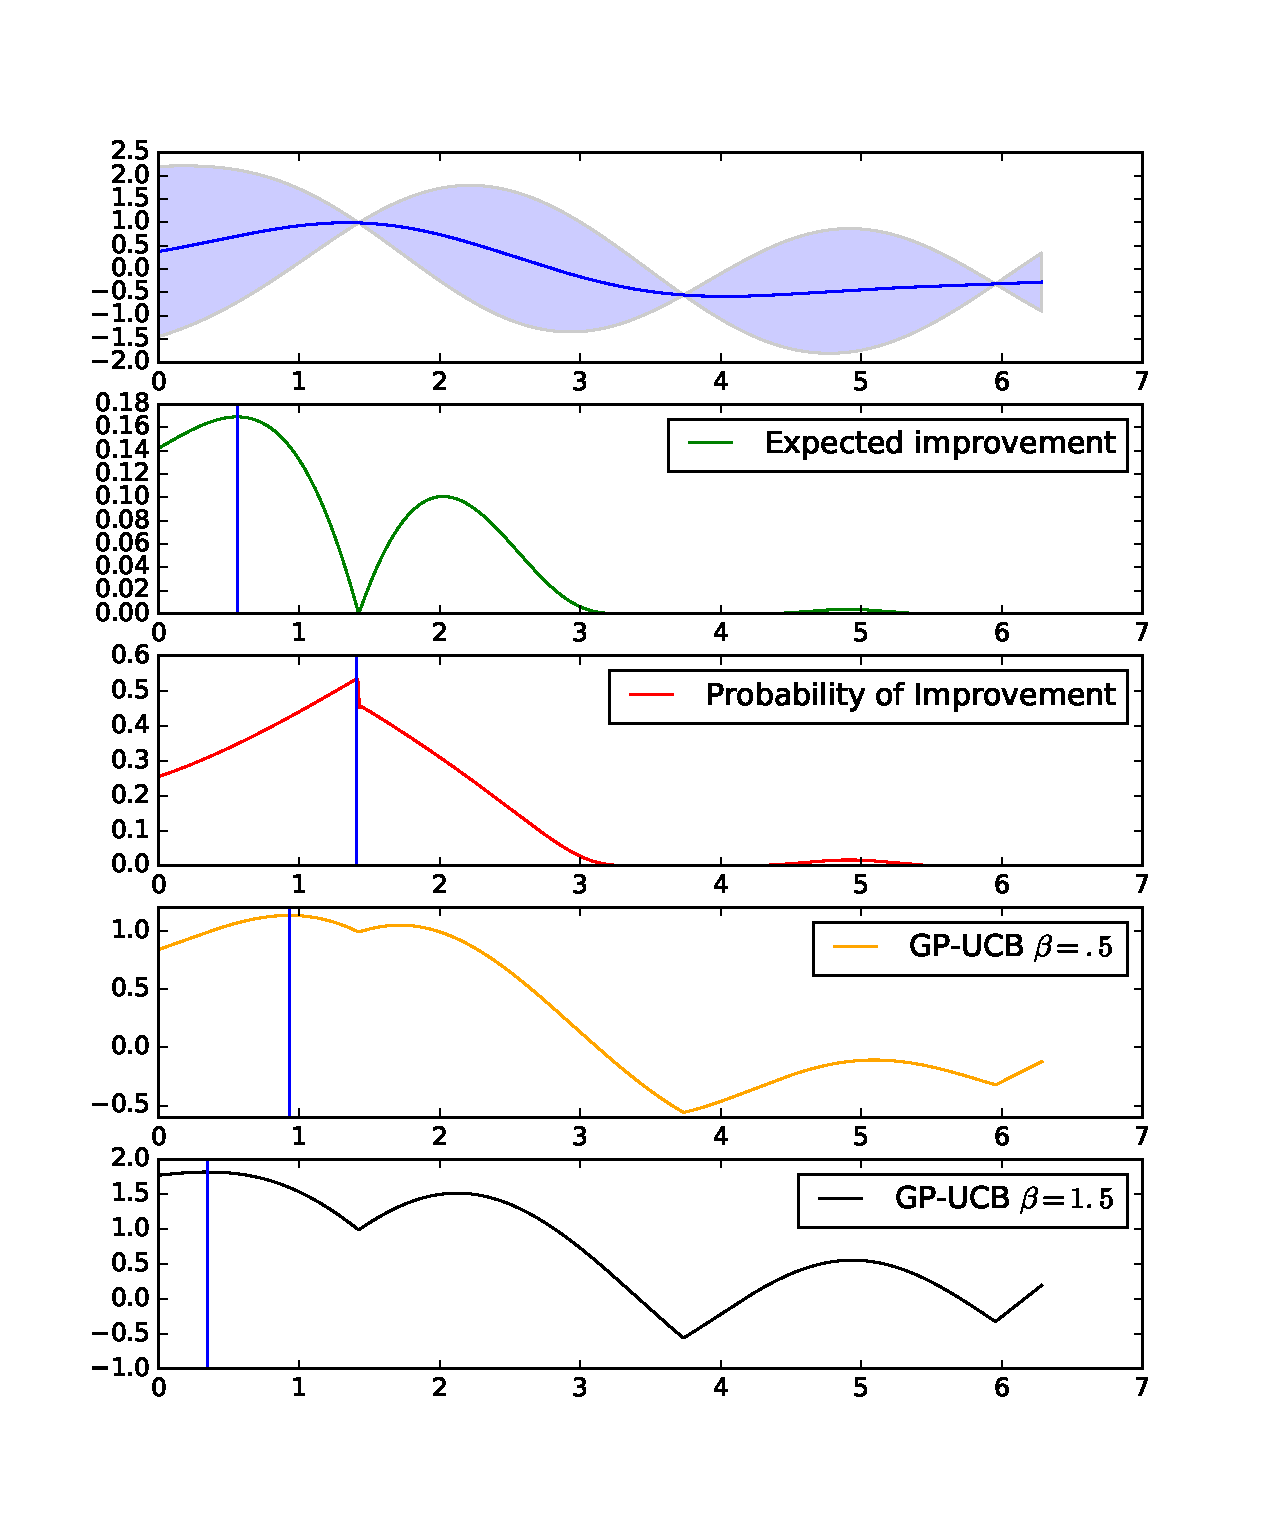
\includegraphics[scale=.6]{figures/chapter3/acqzoo}
\end{figure}

\subsection{Why does Bayesian Optimization work?}

In this small section, we will consider very briefly why the Bayesian Optimization procedure is efficiently making use of the information provided by the mean and variance posterior distribution of the GP. The explanation is mostly visual by means of Figure \ref{fig:explanation}. The plot shows a Gaussian Process regression model, as well as its confidence interval, comprised from a lower confidence bound $L = \mu(\boldsymbol{x}) - q\sigma(\boldsymbol{x})$ and an upper confidence bound $U = \mu(\boldsymbol{x}) + q\sigma(\boldsymbol{x})$ for a quantile $q>0$.\\

In practice, when we are interested in doing hyperparameter search in machine-learning, the algorithms are very blunt, in the sense that the most common strategies explore the entire space, either exhaustively or randomly. The acquisition functions defined in this chapter before use information from the Gaussian Process prior to explore efficiently the space. The specifics of each acquisition function have already been discussed, specially their exploration/exploitation balance, but they all share some common logic.\\

Bayesian Optimization is efficient because it ignores all the space where the predicted upper confidence bound is lower than the maximum value of the lower confidence bound. It only uses the space that fulfills this criteria, according to the strategy selected by the chosen acquisition function. This remains a very reasonable assumption throughout the whole optimization procedure. The code for generating this particular representation can be consulted in Appendix \ref{bayoptwork}.

\begin{figure}
	\caption{A visual explanation on why Bayesian optimization is efficient at exploring the space. It ignores all the input space where the UPB is lower than the point with maximum LCB.}
	\label{fig:explanation}
	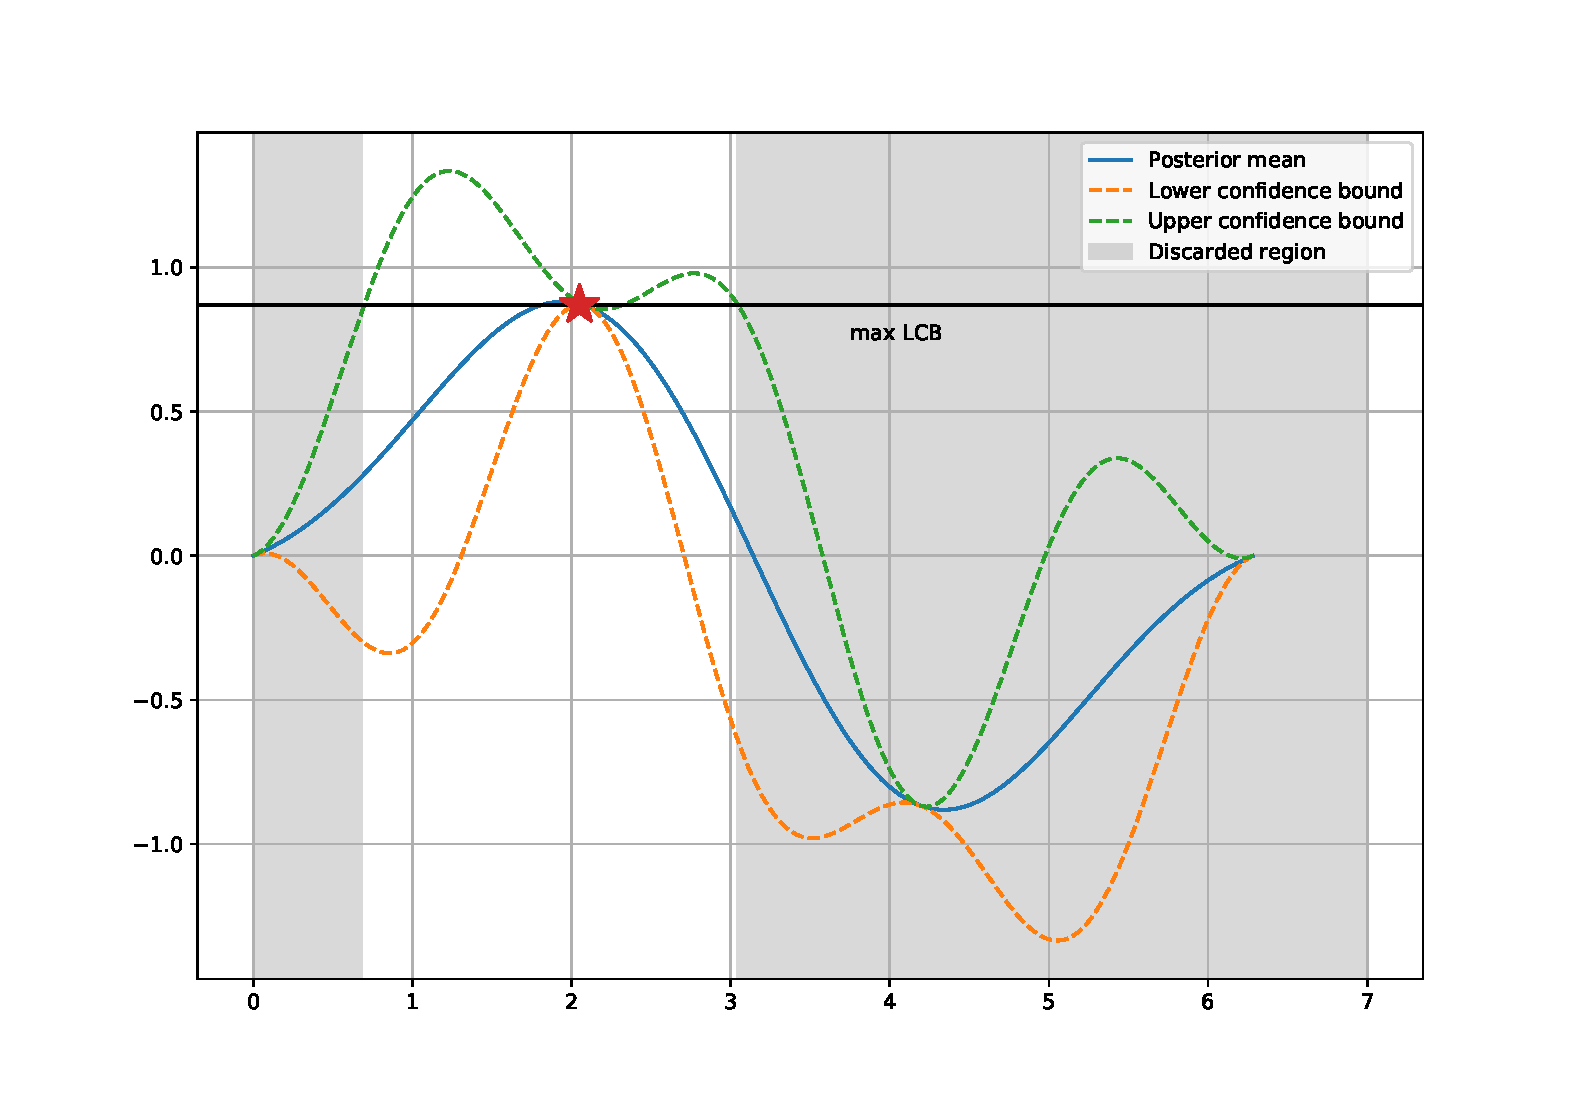
\includegraphics[width=\textwidth]{figures/chapter3/explanation}
\end{figure}


\section{Role of GP hyperparameters in optimization}

We already considered the role of hyperparameters in Gaussian Process regression in section \ref{hyper}. However, one may wonder how the estimation of this parameters, one way or another may affect the optimization procedure. So far, we have assumed that during the optimization procedure, parameters $\theta$ were given. Here we will consider two ways of handling hyperparameters during the optimization procedure, the one we presented, type II maximum likelihood estimation and approximate marginalization. For the moment, consider a generic acquisition function $\alpha:\mathcal{X} \times \Theta \rightarrow \mathbb{R}$, where $\theta \in \Theta$ are our Gaussian Process hyperparameters. Naturally, one wishes to marginalize the uncertainty caused by $\theta$ with the following expression:

\begin{equation}
\alpha(\boldsymbol{x}) = \mathbb{E}_{\theta|\mathcal{D}_n}\left[ \alpha(\boldsymbol{x}, \theta) \right] = \int_{\Theta} \alpha(\boldsymbol{x}|\theta)p(\theta|\mathcal{D}_n)d\theta.
\end{equation}

The simplest way to do this is what we saw in \ref{posteriorhyper}, to optimize the marginal log-likelihood to obtain MAP estimates $\hat{\theta}_{\mathrm{MAP}}$. Then, in each step of the optimization procedure, we simply maximize:

\begin{equation}
\hat{\alpha}(\boldsymbol{x}) = \alpha(\boldsymbol{x}, \hat{\theta})
\end{equation}

That is, we optimize the acquisition function defined by the \textit{optimal} hyperparameters for the Gaussian Process determined in each step. Again, optimizing the marginal log-likelihood is a problem of its own, but it is common to use quasi-Newton methods such as L-BFGS-B methods.\\

A more Bayesian approach is to incorporate the uncertainty of $\theta$ into our model, since it may have an important role in guiding exploration. Point estimates are in a sense \textit{winners} that may not capture the complexity of the response surface. The second approach we will be considering here, will be therefore to marginalize out hyperparameters using Markov Chain Monte Carlo (MCMC) sampling techniques. In practice, we will need to average $M$ samples $\left\lbrace\theta_n^{(i)}\right\rbrace ^{M}_{i=1}$ from the posterior distribution $p(\theta|\mathcal{D}_n)$.

\begin{equation}
\mathbb{E}_{\theta|\mathcal{D}_n}\left[ \alpha(\boldsymbol{x},\theta )\right] \approx \sum_{i=1}^M \alpha(\boldsymbol{x},\theta_n^{(i)})
\end{equation}

Since it is not possible to have an analytical expression for the posterior distribution $p(\theta|\mathcal{D}_n)$, it is common to use MCMC techniques like Hamiltonian Monte Carlo [ref] to produce a sequence of samples whose stationary distribution is the posterior we are looking for. Once $M$ valid samples are obtained, they are evaluated in the acquisition function and averaged. Quadrature methods can be used instead of MCMC techniques, yielding a weighted mixture:

\begin{equation}
\mathbb{E}_{\theta|\mathcal{D}_n}\left[ \alpha(\boldsymbol{x},\theta )\right] \approx \sum_{i=1}^M \omega_i \alpha(\boldsymbol{x},\theta_n^{(i)})
\end{equation}

However, and to finish this section, in the problems that we will tackle in the experiments, it is usually a bad idea to estimate kernel hyperparameters. Estimating these hyperparameters with few function evaluations is a very challenging task, and can lead to disastrous results, as proven in [ref]. The marginal log-likelihood surface can easily fall into traps or be very flat, as seen by the (not cherry-picked) example in Figure \ref{fig:logmarginal}. Even the more advanced MCMC or quadrature methods still suffer from this problem.

\section{Optimizing the acquisition function}

We have presented many acquisition functions in this chapter and provided a simple example to demonstrate basic functionality. However, so far, we have assumed that the acquisition function can be easily optimized. This is however, a problem of its own. The reader may be thinking that we have, in fact, changed one optimization problem (the one where we are interested in optimizing $f$) for another! (in which we now have to optimize $\alpha$). This is technically true, but bear in mind that while $f$ is very expensive to evaluate, $\alpha$ is very cheap, and it is reasonable to spend a bit more computational effort in evaluating $\alpha$ if it implies having to evaluate $f$ less.\\

Maximizing $\alpha$, however, is not an easy task. The acquisition function is often multi-modal and therefore non-convex, as it can be see again in Figure \ref{fig:acqzoo}. Theoretical convergence, furthermore, is only guaranteed when the optimal point $\boldsymbol{x}^*$ in the acquisition function is found [ref]. At the end of the day, we encounter yet another global optimization problem that needs to be solved. From a practical point of view, there are many approaches the community has taken to solve this problem, from discretization [ref], adaptive-grids [ref]. If gradient information is available (rarely the case), a multi-start gradient ascent approach can be taken [ref]. Evolutionary approaches like CMA-ES can also be used [ref]. pyGPGO, in the \texttt{GPGO} module uses by default a multi-start quasi-Newton method (L-BFGS-B) to optimize the acquisition function, which in practice seems to work reasonably well. A CMA-ES optimizer interface is also available for the user.\\

Other methods have been proposed as alternatives to Bayesian Optimization in this aspect. [ref], sequentially building space-partitioning trees by splitting leaves with high function values or upper confidence bounds. This is called \textit{Simultaneous Optimistic Optimization} (SOO) [ref]. Though these algorithms do not require any auxiliary information (smoothness) or optimization, it has been shown that they do not perform quite as competitively as the Bayesian optimization framework, especially when prior knowledge is available. 

\section{Computational costs}

Remember from chapter 2 that Gaussian Process regression has analytical expressions for the mean and variance of the posterior process. However, this exact inference is $O(n^3)$, where $n$ is the number of training samples. This is caused by the inversion of $K$. pyGPGO uses a Cholesky decomposition that once computed, can reduce the cost of predicting to $O(n^2)$. If during the search procedure, however, we change $K$, for example, due to hyperparameter optimization, this $O(n^3)$ order is unavoidable for the traditional framework. Several approaches have been explored in the literature for approximating the output of the analytical solution. Mainly, there are two types of solutions, those that try to sparsify the process and those that use another type of surrogate model, such as Random Forests.\\

\subsection{Approximations to the analytical GP. Alternative surrogates.}

One of the first solutions is the \textit{Sparse pseudo-input Gaussian Processes} (SPGP) [ref]. This is a straightforward approach to model large $n$ using $m < n$ pseudo-inputs to reduce the rank of the covariance matrix to $m$. This method forces the interaction between the $\boldsymbol{x}_{1:n}$ data points and test points $\boldsymbol{x}_*$ inducing $m$ pseudo-inputs, achieving an approximate posterior in $O(nm^2 + m^3)$. Let $\boldsymbol{f}$ and $\boldsymbol{f}_*$ denote two sets of latent function (them being our training and testing points respectively). The assumption is that $\boldsymbol{f} and \boldsymbol{f}_*$ are independent given a third set of variables $\boldsymbol{u}$, that is:

\begin{equation}
p\left(\boldsymbol{f}_*, \boldsymbol{f}\right) = \int p(\boldsymbol{f}_*, \boldsymbol{f}, \boldsymbol{u})\; d\boldsymbol{u} \approx \int q(\boldsymbol{f}_*|\boldsymbol{u})q(\boldsymbol{f}|\boldsymbol{u})p(\boldsymbol{u})\; d\boldsymbol{u} = q(\boldsymbol{f}, \boldsymbol{f}_*) 
\end{equation}

where $\boldsymbol{u}$ is a vector representing the function values at the pseudo-inputs. Different pseudo-input Gaussian Process pseudo-input approximations specify their own form of $q(\boldsymbol{f}|\boldsymbol{u})$ and $q(\boldsymbol{f_*|u})$ training and test conditionals. [ref]. How to choose the locations of these pseudo-inputs is another problem, is is usually done by maximizing the marginal log-likelihood of the SPGP [ref]. Another approach uses variational inference [ref] to marginalize the pseudo-inputs to maximize the fidelity to the original Gaussian Process. It has been noted, however, that the computational savings of the pseudo-input methods impact heavily variance estimates. In the Bayesian optimization framework, this variance of the posterior predictive distribution is heavily used to guide exploration, so this behavior is undesirable.\\

Another approach is named \textit{Sparse spectrum Gaussian Processes} (SSGP). Using the ideas of pseudo-input methods, these methods apply the same concept in kernel spectral space. [ref]. From basic spectral analysis, Bochner's theorem states that a stationary kernel $k(\boldsymbol{x}, \boldsymbol{x}_*)$ defines a positive finite Fourier spectrum $s(\boldsymbol{\omega})$:

\begin{equation}
k(\boldsymbol{x}) = \dfrac{1}{(2\pi)^d}\int e^{-i\boldsymbol{\omega}^T\boldsymbol{x}}s(\boldsymbol{\omega}) d\boldsymbol{\omega}
\end{equation}

We can normalize this spectrum to make it a valid probability density function, such as $p(\boldsymbol{\omega}) = \dfrac{s(\boldsymbol{\omega})}{\nu}$. Now evaluating the kernel is the same as the expectation of the Fourier basis with respect to $p(\boldsymbol{\omega})$:

\begin{equation}
k(\boldsymbol{x}, \boldsymbol{x_*}) = \nu \mathbb{E}_{\boldsymbol{\omega}}\left[ e^{-i\boldsymbol{w}^T(\boldsymbol{x} - \boldsymbol{x}_*)}   \right]
\end{equation}

Monte Carlo techniques can be used to approximate this expectation using $m$ samples from the spectral density, so that:

\begin{equation}
k(\boldsymbol{x}, \boldsymbol{x_*}) \approx \dfrac{\nu}{m}\sum_{i=1}^m e^{-i\boldsymbol{\omega}_{(i)}^T\boldsymbol{x}} e^{-i\boldsymbol{\omega}_{(i)}^T\boldsymbol{x_*}} 
\end{equation}

where $\boldsymbol{\omega}_{(i)} \sim s(\boldsymbol{\omega})/\nu$. The computational cost in this approach can be reduced to $O(nm^2 + m^3)$. It has been noted [ref] for this approximation method that whereas the uncertainty estimates are smoother than with the pseudo-input methods, observations away from the observed values exhibit irregular variance estimates. This again is undesirable behavior in the Bayesian Optimization framework.\\

As an alternative, several authors [ref] have suggested using different surrogate models in the Bayesian Optimization framework. Special attention has been drawn towards the Random Forest regression model, in the context of sequential model-based algorithm configuration. Random Forests are a very popular choice in the machine-learning community with very successful results in practice. They were introduced in 2001 by [ref], being an ensemble bagging tree-based method. Random Forests allow for training using sub-samples of data, giving it the ability to scale to large evaluation budgets, where exact analytical Gaussian Process regression would be infeasible in practice. The exploration strategy requires an uncertainty estimation for prediction at test points to apply the Bayesian optimization framework. The empirical variance in the predictions across trees was proposed as a substitute. This heuristic has been shown to work in practice [ref].\\

Random Forests are known to provide very good estimates when doing \textit{interpolation} of seen data (or in its neighbourhood), they are very poor \textit{extrapolators}. On points far from training data, the predictions across all trees in the model are very similar, providing poor predictions and more importantly, providing extremely confident (but erroneous) variance estimates. While Gaussian Processes are also terrible extrapolators, they produce reliable variance estimations far from training data, yielding better estimates for exploration and exploitation in the framework.

\subsection{Parallelization}

The Bayesian Optimization framework is inherently a sequential decision problem, where each candidate point to sample is selected after fitting a Gaussian Process to the currently available data. However, and given the parallel nature of current CPU architectures, significant speed-ups in clock time can be achieved if they are made good use of. That implies evaluating the acquisition function in parallel. While not entirely parallel in nature, some authors have proposed approaches based on the imputation of yet-to-run evaluations. Given $\mathcal{D}_n = \left\lbrace (\boldsymbol{x}_n, y_n) \right\rbrace$ known data and $\mathcal{D}_p = \left\lbrace \boldsymbol{x}_p \right\rbrace$ remaining to evaluate data, an idea is to impute the latter, $\hat{\mathcal{D}}_p = \left\lbrace (\boldsymbol{x}_p, \hat{y}_p) \right\rbrace$, and then use the typical Bayesian optimization framework on the augmented data $\mathcal{D}_n \cup \hat{\mathcal{D}}_p$.\\

Simple strategies have been proposed over time. The \textit{constant liar} strategy proposes $\hat{y}_p = c, \forall p$, where $c \in \mathbb{R}$ is a predefined constant. Other strategies like the \textit{kriging believer} uses the Gaussian Process posterior predictive mean instead: $\hat{y}_p = \mu_n(\boldsymbol{x}_p)$. More complex approaches have been proposed instead, for example [ref] proposed the use of $s$ fantasies sampled from each unfinished experiment (out of a total of $J$) from the full GP posterior predictive distribution. Then they are averaged in a Monte Carlo fashion:

\begin{align}
\alpha(x, \mathcal{D}_n, \mathcal{D}_p) =& \int_{\mathbb{R}^J} \alpha(x, \mathcal{D}_n \cup \hat{\mathcal{D}_p})P(\hat{y_{1:J}}, \mathcal{D}_n) dy_{p, 1:J}\\
&\approx \dfrac{1}{S} \sum_{i=1}^S \alpha(x, \mathcal{D}_n \cup \hat{\mathcal{D}}_p^{(s)})
\end{align} 

and $\hat{\mathcal{D}}_p^{(s)} \sim P(\hat{y}_{1:J}, \mathcal{D}_n)$. [ref] has demonstrated empirically that this approach works reasonably well when $\alpha$ is chosen to be the Expected Improvement acquisition function. Other attempts [ref] have also been made using GP-UCB. Note that while these approaches are valid, they are not parallel per se. A true parallel approach to Bayesian optimization would propose simultaneously a set of candidates, or would use the information of posterior Gaussian Processes computed in another thread to make the sequential decision. 


\section{Step-by-step examples}

We have explored the basics of Gaussian Process regression and Bayesian Optimization by now. To provide a more thorough understanding on the logic behind Algorithm \ref{bayesopt}, we will provide two different examples in this section. While not very complex, they serve illustrative purposes on how the optimization framework works. We hope this section will clear any practical consideration on how the procedure selects the next point to sample, graphically.

\subsection{Optimizing the sine function}

Again, it is no surprise for the reader that we choose the sine function as our first example to provide an intuition on how the Bayesian Optimization framework works step-by-step. We will be optimizing our function within the boundaries $x \in [0, 2\pi]$, where we know an optima is exactly at $x^* = \pi/2$. This example is particularly interesting to see how the next point is chosen balancing exploration and exploitation of the acquisition function. Now, as in most practical cases throughout this thesis, we will use the Expected Improvement acquisition function. The step-by-step optimization procedure for 6 complete epochs can be checked in Figure \ref{fig:1dstep}. The code to produce these Figures can be checked in Appendix \ref{sineopt}.\\

It can be appreciated that the chosen acquisition function leverages achieves a very reasonable compromise between mean and variance in the first stages of optimization, but exploits heavily in steps 3 and 4. It tries to explore again in step 5, and comes back to exploit at the end of the procedure.


\begin{figure}
	\centering
	\caption{Six complete optimization epochs in the Bayesian Optimization framework for the target sine function in $x\in [0, 2\pi]$.}
	\label{fig:1dstep}
	\begin{subfigure}[b]{0.45\textwidth}
		\caption{Step 1}
		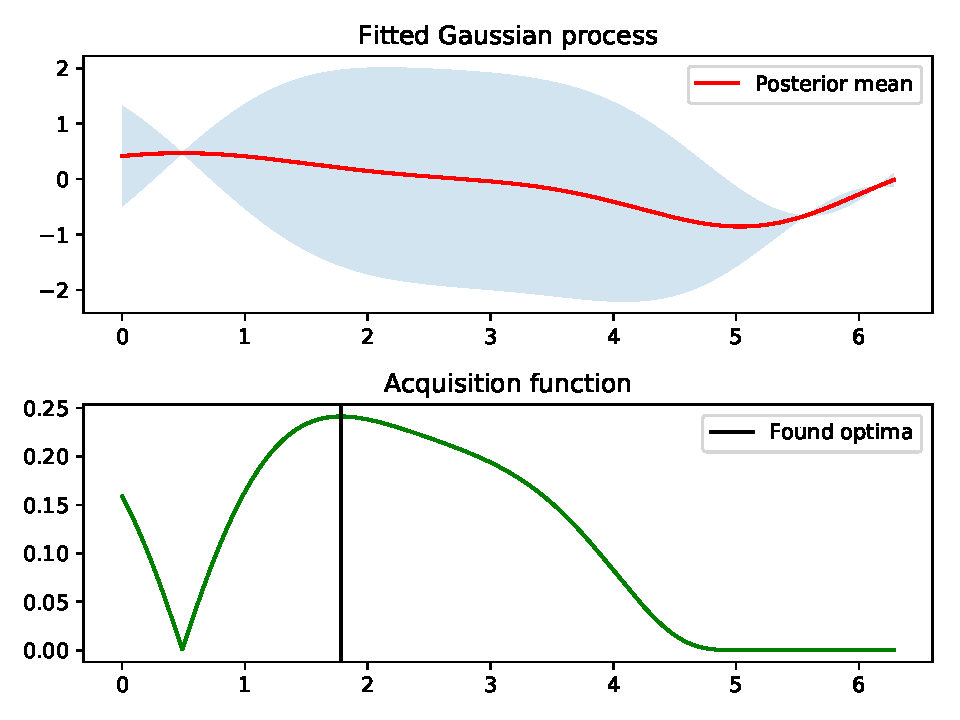
\includegraphics[width=\textwidth]{figures/chapter3/sine/0.pdf}
	\end{subfigure}
	\begin{subfigure}[b]{0.45\textwidth}
		\caption{Step 2}
		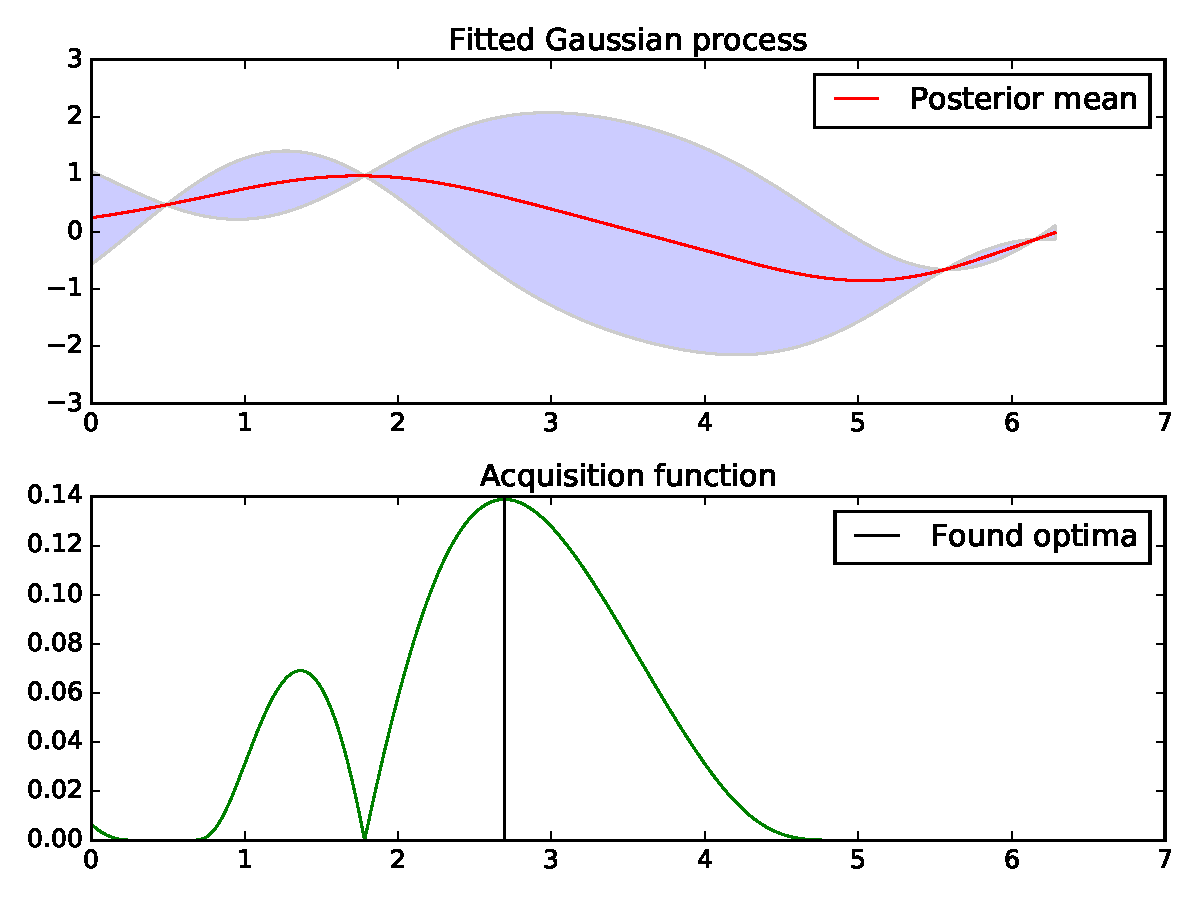
\includegraphics[width=\textwidth]{figures/chapter3/sine/1.pdf}
	\end{subfigure}
	
	\begin{subfigure}[b]{0.45\textwidth}
		\caption{Step 3}
		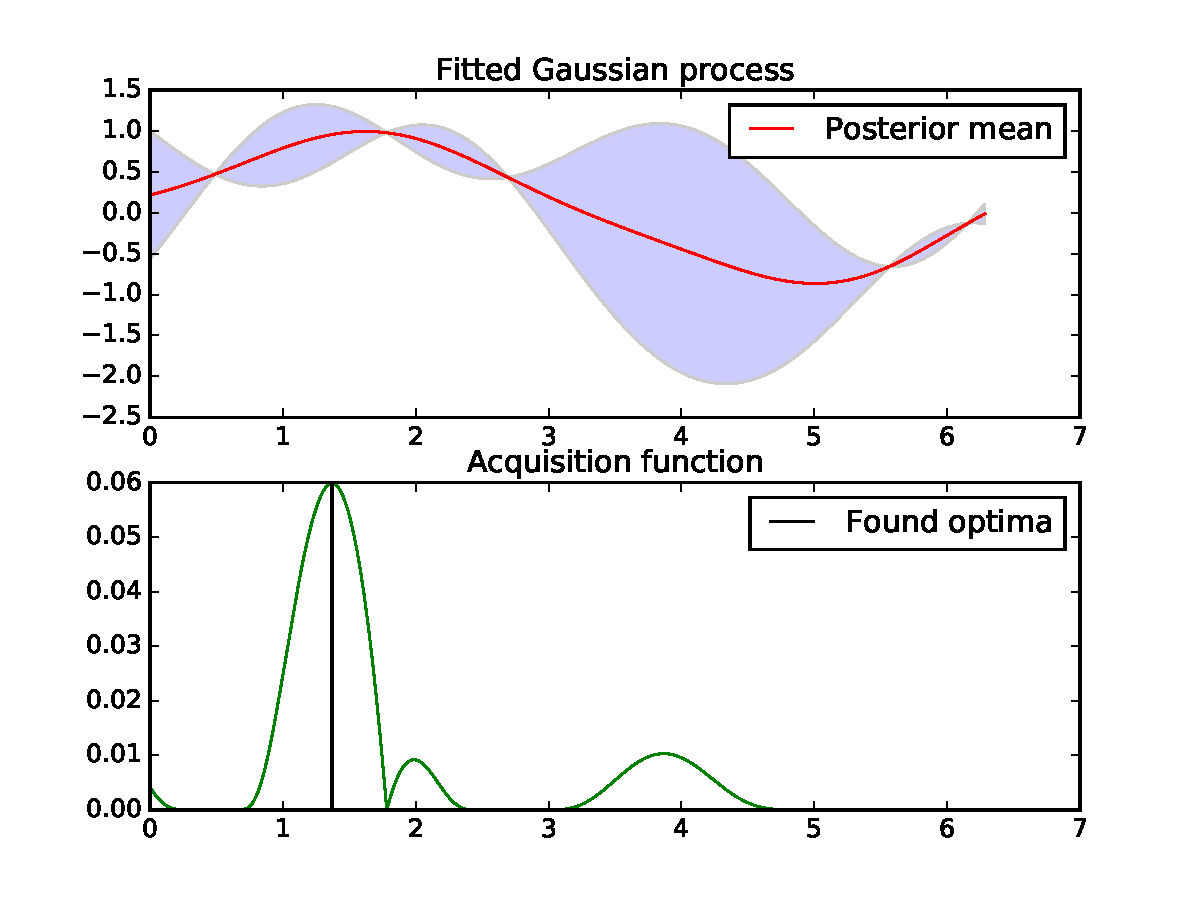
\includegraphics[width=\textwidth]{figures/chapter3/sine/2.pdf}
	\end{subfigure}
	\begin{subfigure}[b]{0.45\textwidth}
		\caption{Step 4}
		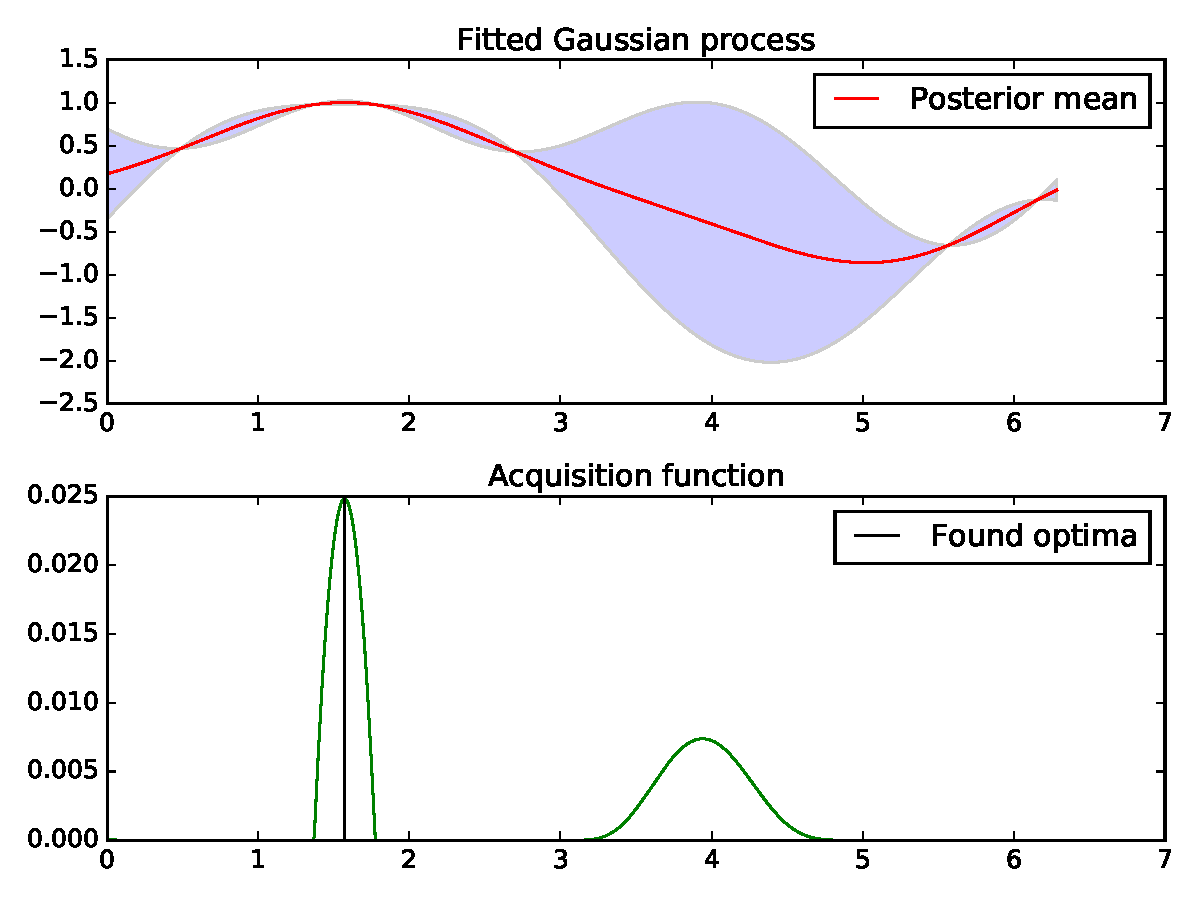
\includegraphics[width=\textwidth]{figures/chapter3/sine/3.pdf}
	\end{subfigure}
	
	\begin{subfigure}[b]{0.45\textwidth}
		\caption{Step 5}
		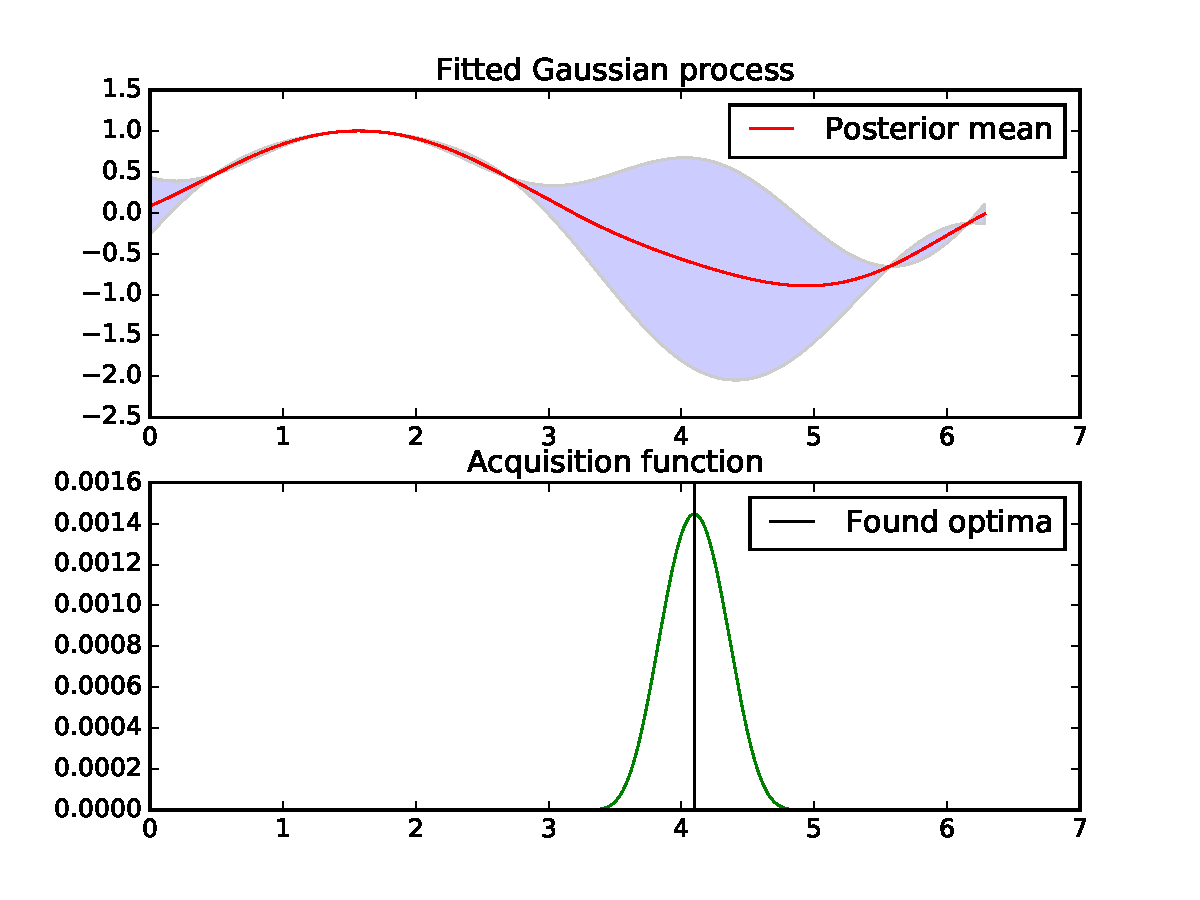
\includegraphics[width=\textwidth]{figures/chapter3/sine/4.pdf}
	\end{subfigure}
	\begin{subfigure}[b]{0.45\textwidth}
		\caption{Step 6}
		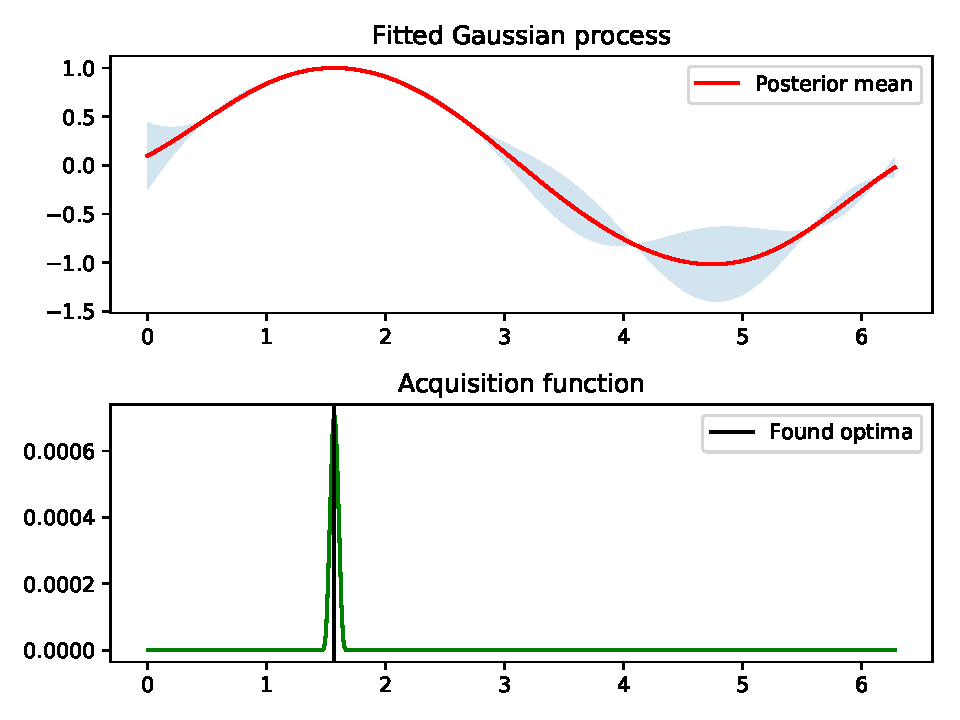
\includegraphics[width=\textwidth]{figures/chapter3/sine/5.pdf}
	\end{subfigure}
\end{figure}


\subsection{Optimizing the Rastrigin function}

In this example, we will try to optimize the two-dimensional Rastrigin function:

\begin{equation}
f(x, y| a, b) = (a - x)^2 + b(y - x^2)^2
\end{equation}

For given hyperparameters $a=1,\, b=100$ and in a bounding box defined by $x,y \in [-1, 1]$. A biplot of this function can be checked in Figure \ref{fig:rosen}. This particular version of the Rossenbrock function has four different local optima, therefore it is multimodal. We would expect our GPGO algorithm to converge to one of these optima, while still exploring the space at earlier stages of optimization.\\

\begin{figure}
	\centering
	\caption{A 2D representation of the Rossenbrock function for $x, y \in [-1, 1]$.}
	\label{fig:rosen}
	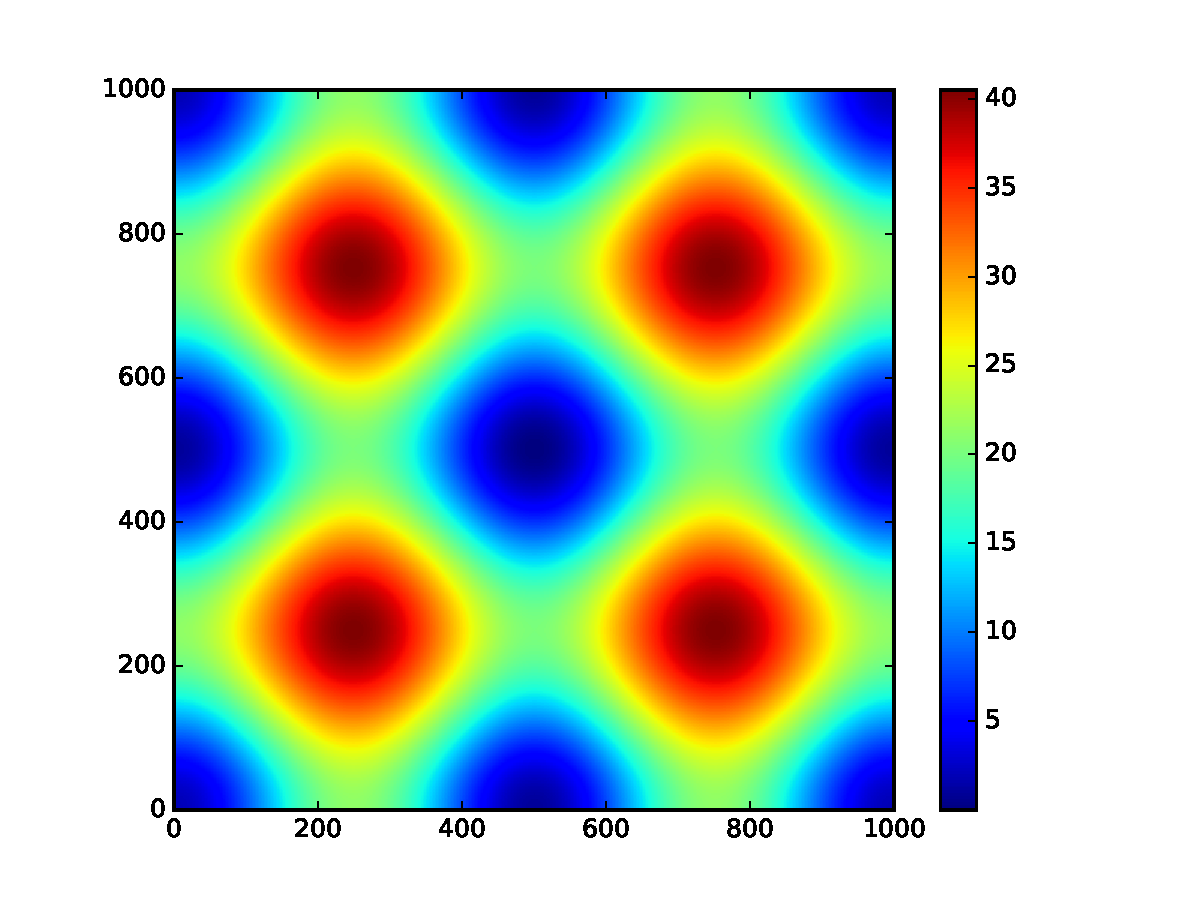
\includegraphics[scale=0.5]{figures/chapter3/rosen/rosen}
\end{figure}

Given the low-dimensional space we are optimizing, we will plot the posterior mean and variance of the Gaussian Process, as well as the acquisition function. Again, the Expected Improvement acquisition function is used. The complete step-by-step optimization procedure for 6 epochs can be seen in Figure \ref{fig:2dstep}. For a more visually appealing explanation of the same procedure, there is a video in the associated GitHub repository of this thesis. The code to generate these figures is available in Appendix \ref{rastriginopt}.\\

It can be seen that during the previous steps before fitting a Gaussian Process, that a random evaluation is reasonably close to one of the optima. This causes the acquisition function to exploit that area in the first step. In the second step, however, it starts exploring the area that is close to a second local optima, mostly because it is a large-variance area. It exploits in the third step, and keeps exploring the rest of the space during the following stages, therefore efficiently balancing exploitation and exploration as intended in the optimization procedure.

\begin{figure}
	\centering
	\caption{Six complete optimization epochs in the Bayesian Optimization framework for the target Rossenbrock 2D function.}
	\label{fig:2dstep}
	\begin{subfigure}[b]{0.45\textwidth}
		\caption{Step 1}
		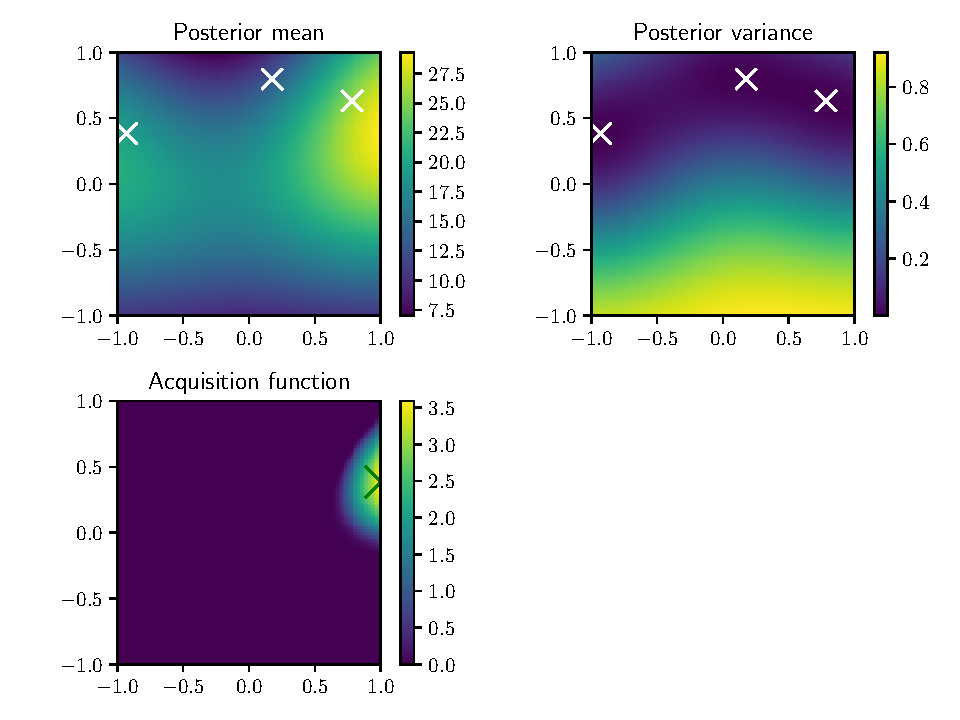
\includegraphics[width=\textwidth]{figures/chapter3/rosen/0.pdf}
	\end{subfigure}
	\begin{subfigure}[b]{0.45\textwidth}
		\caption{Step 2}
		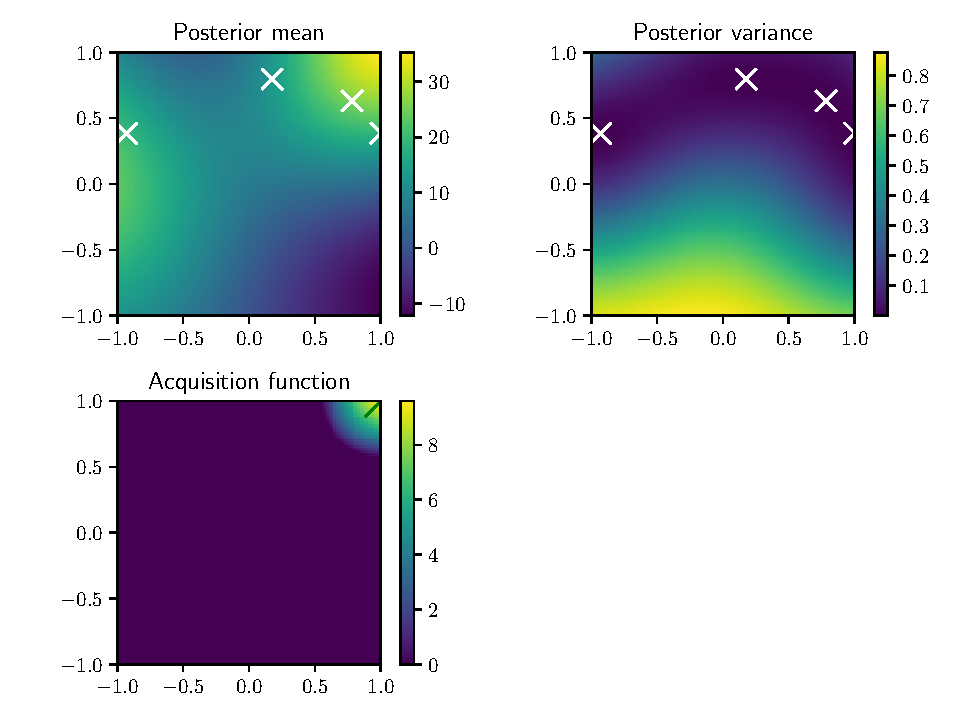
\includegraphics[width=\textwidth]{figures/chapter3/rosen/1.pdf}
	\end{subfigure}
	
	\begin{subfigure}[b]{0.45\textwidth}
		\caption{Step 3}
		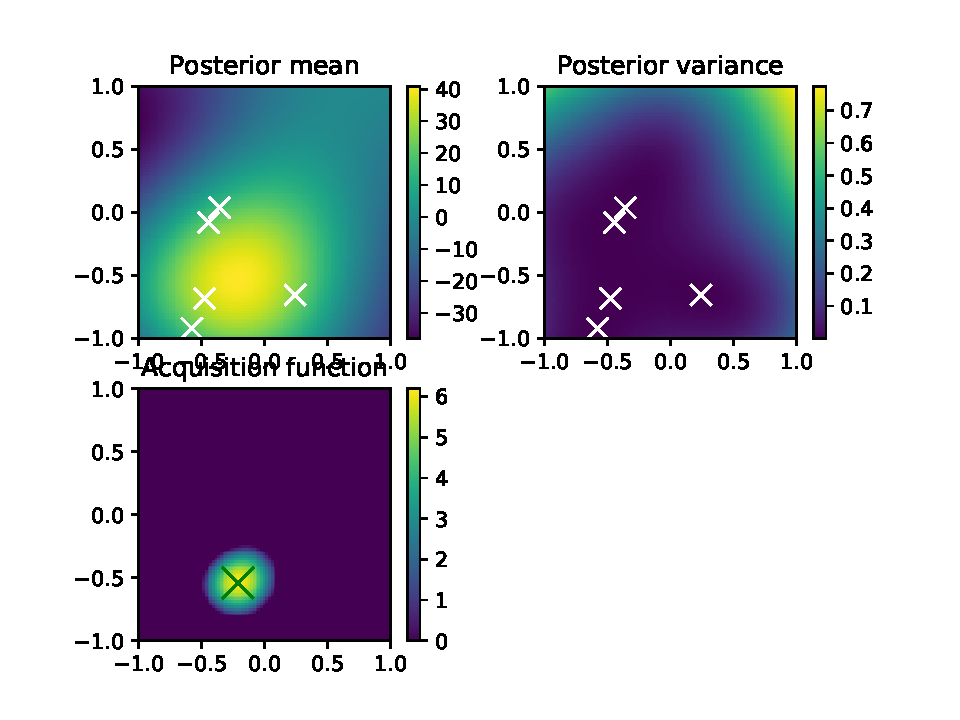
\includegraphics[width=\textwidth]{figures/chapter3/rosen/2.pdf}
	\end{subfigure}
	\begin{subfigure}[b]{0.45\textwidth}
		\caption{Step 4}
		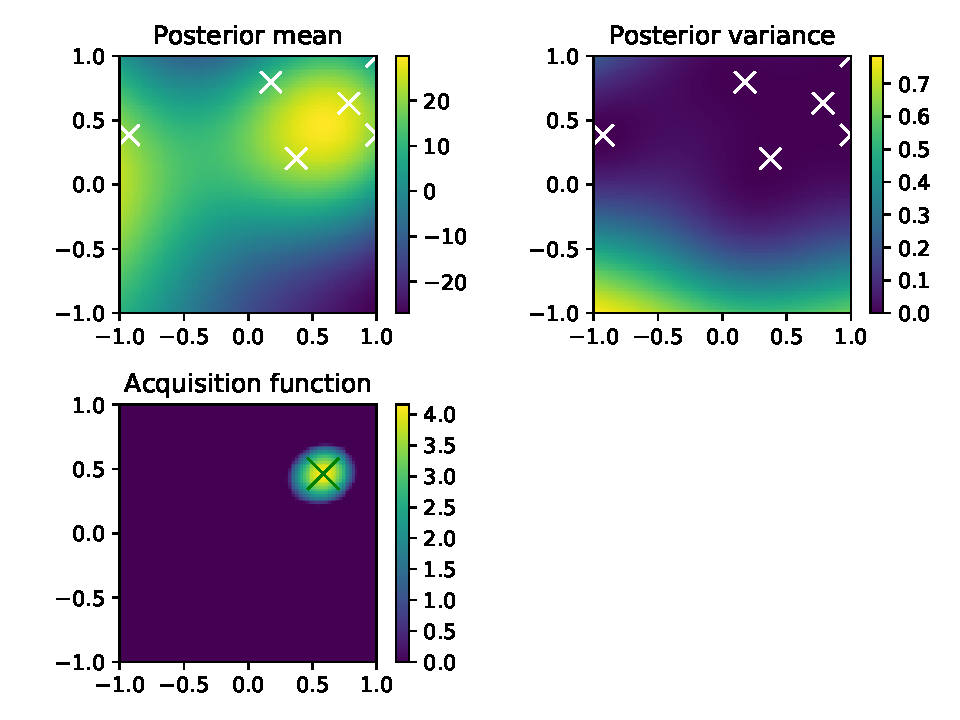
\includegraphics[width=\textwidth]{figures/chapter3/rosen/3.pdf}
	\end{subfigure}
	
	\begin{subfigure}[b]{0.45\textwidth}
		\caption{Step 5}
		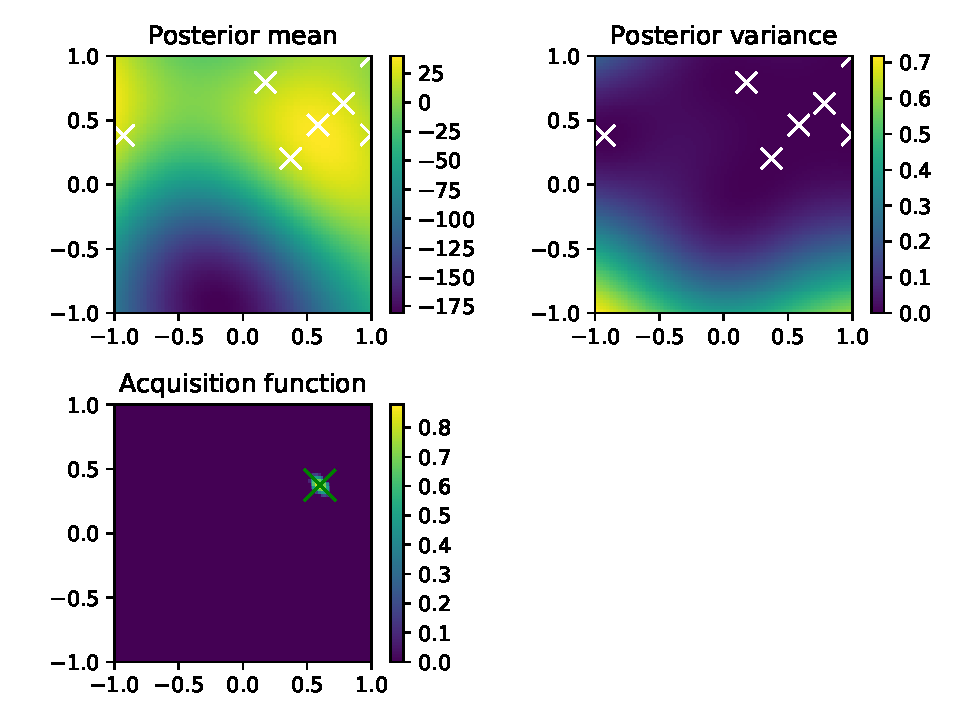
\includegraphics[width=\textwidth]{figures/chapter3/rosen/4.pdf}
	\end{subfigure}
	\begin{subfigure}[b]{0.45\textwidth}
		\caption{Step 6}
		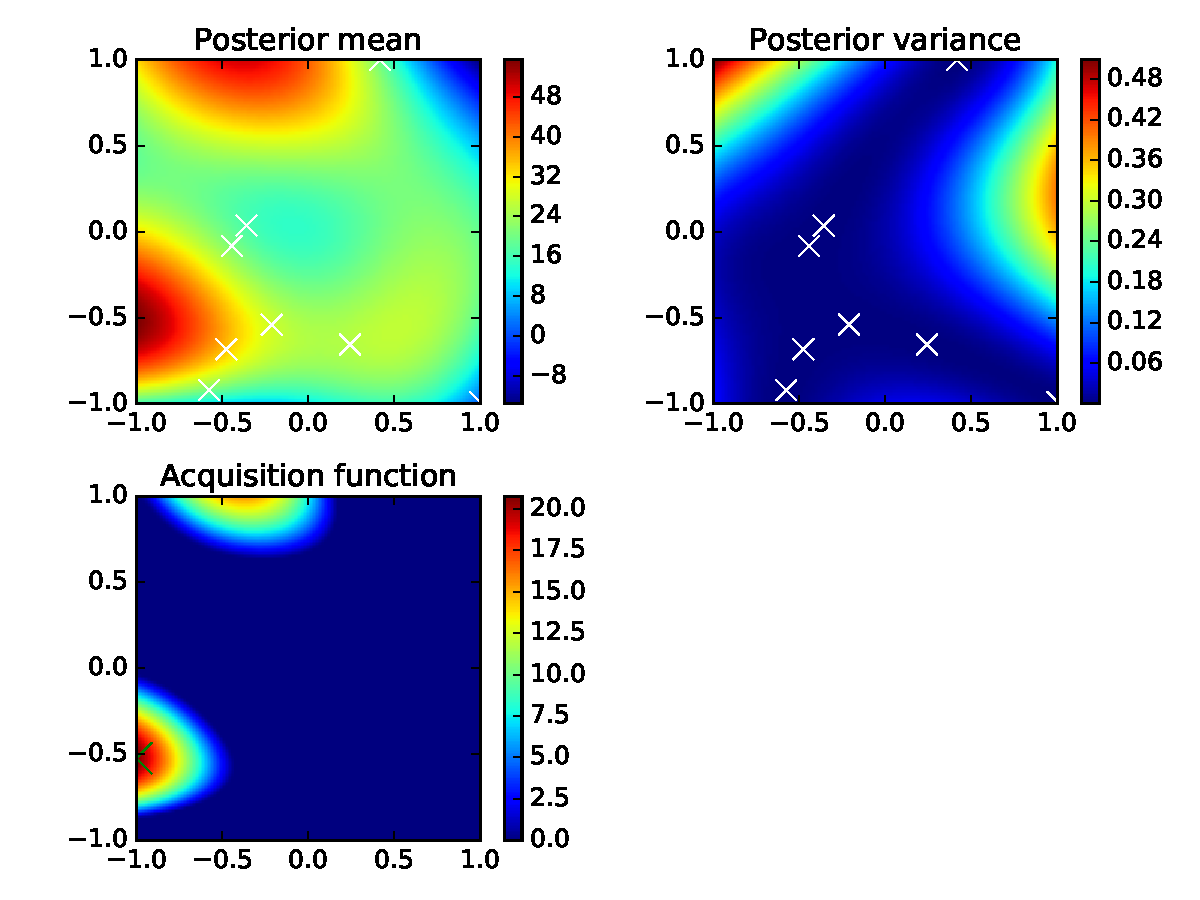
\includegraphics[width=\textwidth]{figures/chapter3/rosen/5.pdf}
	\end{subfigure}
\end{figure}

\chapter{Experiments}

In this chapter we will expose all the results using all implemented code for Gaussian Process regression and Bayesian Optimization in pyGPGO. First, we start by providing some benchmarking rules, how performance shall be evaluated across different models and datasets. In general, the models presented here hopefully span enough diversity: support vector machines , neural networks and bagging/boosting methods are among these candidates. Datasets come from very different research areas, spanning from biophysics to medicine. Some datasets will span an entire section, explaining the rationale behind the problem, while results for others will be briefly discussed. We hope to show here that Bayesian Optimization works reasonably well for hyperparameter optimization of machine-learning models, and can outperform other well known strategies in the majority of cases.


\section{Benchmarking rules}
\subsection{Other strategies for hyper-parameter optimization}

Hyper-parameter optimization is usually the most tedious part in fitting a machine-learning algorithm. In practice, we are interested in models whose loss, evaluated on an independent part of data is as low as possible. Different hyper-parameter choices lead to different losses, therefore finding the optimal set is of importance. In reality, we will never know that the point found is the global optimum, but from a practical point of view, we are only interested in finding the model that works best in a production setting.\\

In the machine-learning community, hyper-parameter optimization is often overlooked, and in fact, some of the most famous models (e.g. Random Forests) have been shown to be somewhat insensitive to hyper-parameter optimization [ref]. Four common strategies for finding \textit{better} hyper-parameters are presented here: grid search, random search, simulated annealing and gradient-based methods. Only random search and simulated annealing will be compared against our Bayesian Optimization algorithm, as implemented in pyGPGO. Details on how these work are laid down below:

\begin{itemize}
	\item \textbf{Grid search}. Also known as parameter sweep. This is simply an exhaustive search in a user specified subset of parameter space. Search bounds have to be set manually. When multiple hyper-parameters have to be optimized over their sets, grid search considers the Cartesian product of all of them. This poses a problem when the number of hyper-parameters to optimize grows, also known as the curse of dimensionality. While suffering from this problem, grid search is still widely used for small to mid-sized problems, where function evaluations are not very expensive. Also, it is embarrassingly parallel: function evaluations can be distributed over in a simple way.
	\item \textbf{Random search}. Grid search is exhaustive since it considers all possible evaluations over a Cartesian product over parameter sets. Randomized search in hyper-parameter space is also a very popular method for the task at hand. In particular, this method has been shown to work considerably better in high-dimensional spaces than grid search [ref]. There is also evidence that often sometimes some hyper-parameters do not affect the loss significantly.
\end{itemize}

\subsection{Evaluation metrics}
\label{evaluation}

Throughout all the experiments, we will be minimizing loss functions, in some form or the other. Every problem presented here is formulated either as a regression or classification task, therefore it is of importance to define early on what type of loss to use in each problem. For binary classification problems, we will use the logarithmic loss, also known as binary cross-entropy, defined by:

\begin{equation}
\mathcal{L}(\boldsymbol{y}, \boldsymbol{\hat{y}}) = -\dfrac{1}{n} = \sum_i \left(y_i \log(\hat{y_i}) + (1 - y_i)\log(1-\hat{y_i})\right)
\end{equation}

The log-loss is very popular among the deep learning folks [ref]. This particular metric does not only take into account whether a classifier makes the right decision given a threshold $c$, (like the 0/1 loss would), but also the confidence in predictions $\boldsymbol{\hat{y}}$. It is also very natural since it is just the negative log-likelihood of a Bernoulli random variable. The use of the logarithm both punishes erroneous extremely confident positive or negative predictions.\\

We generalize the previous metric for multi-class classification problems. The following expression is typically called categorical cross-entropy:

\begin{equation}
\mathcal{L}(\boldsymbol{y}, \boldsymbol{\hat{p}}) = - \dfrac{1}{n} \sum_{i=1}^n\sum_{j=1}^m y_{ij}\log(\hat{p}_{ij})
\end{equation}

where $\hat{p}_{ij}$ is the predicted probability of a sample $i$ belonging to class $j$, and $m$ is the number of classes considered. For continuous regression problems, the loss that we use is the typical mean squared error, defined by:

\begin{equation}
\mathcal{L}(\boldsymbol{y}, \boldsymbol{\hat{y}}) = \dfrac{1}{n} \sum_i \left(y_i - \hat{y_i}\right)^2
\end{equation}

We believe that the losses proposed here are very natural choices in both classification and regression problems.\\

While we have discussed the metrics to evaluate in each predictive problem, we still need to define how these losses will be evaluated in each step. To evaluate the performance of a given hyper-parameter optimization procedure, we have to balance both the performance in terms of loss and the number of evaluations necessary in order to get to a satisfactory solution. In practice, this is exactly how we will benchmark the different strategies, through a plot where the $x$-axis represent the number of function evaluations, and the $y$-axis the best log-loss found.\\

Evaluating the loss function itself can lead to multiple different values depending on the test values. One could choose an approach where this loss is evaluated on a single holdout test. This would lead to noisy estimates, however. We choose the more stable approach of performing a shuffled $k=5$ cross-validation scheme to obtain a more reliable loss estimate. In practice, this means that we fit $5$ models with the same architecture to different train/test splits and average the loss results in each. A total of $n=53$ functions evaluations will be allowed for each strategy in all datasets. This accounts for the fact that the Bayesian Optimization needs at least $3$ function evaluations to fit a surrogate Gaussian Process regressor in the beggining.

\subsection{Bayesian optimization setup}

For all the tests performed with the Bayesian Optimization scheme, we choose the standard squared exponential kernel with a starting default characteristic length-scale $l=1$, signal variance $\sigma_f^2=1$ and noise variance $\sigma_n^2 = 0$. These three hyper-parameters will be continuously adapted using a Type-II Maximum Likelihood approach using gradients during the optimization process, as detailed in Section \ref{empbayes}. Different acquisition functions will be tested in each problem: Expected Improvement, GP-UCB ($\beta= .5$) and GP-UCB ($\beta = 1.5$). All features in all datasets are scaled by default to have zero mean and unit variance.

\subsection{Machine-learning models used}

Since the shape of our objective function depends on both the dataset and the predictor, we try to span as many different types of machine-learning models as possible to provide the most extensive evaluation as possible. Except for rare occasions where we could not fit a model to a particular dataset for numerical conditions, all models are evaluated in all datasets with the same number of parameters and bounds to optimize over.

\section{The binding affinity dataset}

\subsection{Description of the problem}

We will address one of the most popular problems in computational chemistry in this section: protein-ligand binding affinity prediction. The docking procedures (see Figure \ref{fig:docking}) in structural biology typically work as follows: first, by generating a large number of poses of the ligand (a small drug-like molecule compared to the host protein). A pose encompasses position, orientation and conformation of the ligand. Once enough poses are generated, a \textit{scoring function} is in charge of reranking these, that is, its job is to find the correct pose amongst the generated. Correct poses have more \textit{strength} to the binding site of the target than incorrect ones, and this is typically quantified by means of dissociation ($K_d$), inhibition constant ($K_i$) or free energy. These quantities are real valued, and can normally range from $10^{-9}$ to $10^4$ kcal/mol in studies. To account for this very large range of affinities, one typically defines a target variable as $y=-\log_{10}K_{d,i}$ and considers it as a classical regression problem.\\

\begin{figure}
\centering
\caption{Small illustration of the docking procedure. Ligand poses generating by a docking program are ranked according to a given scoring function, hopefully resulting in a valid complex.}
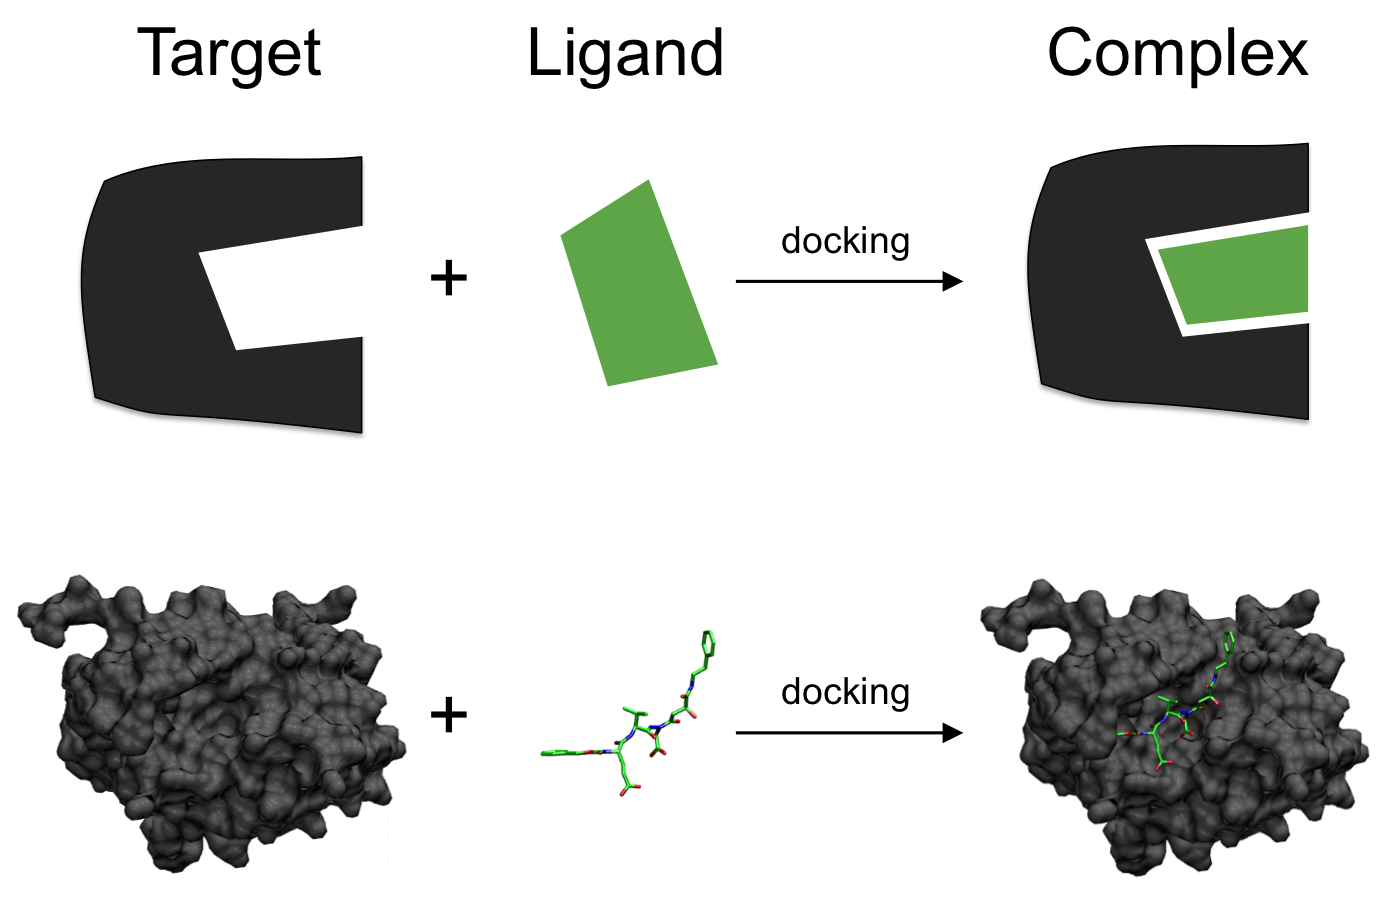
\includegraphics[scale=0.45]{figures/chapter4/docking}
\label{fig:docking}
\end{figure}

While many accurate and reliable algorithms exist for pose generation, the main drawback in docking studies continues to be the scoring function themselves [ref]. This, therefore still is one of the main open problems in computational chemistry. Over the years, plenty of scoring functions have been developed, for which the most common be classified into empirical [ref], force-field based [ref] or knowledge-based [ref]. These \textit{classical} scoring functions do not fully account for certain physical processes that are important for molecular recognition, therefore limiting their ability to rank for some particular protein-ligand binding pairs. Furthermore, each scoring function assumes a particular functional relationship between some variables characterizing the protein-ligand binding complex and their corresponding binding affinity. For example, typical scoring functions can take the form of a weighted sum of physico-chemical properties (as in the case of a Linear Regression (LR) or Partial Least Squares (PLS)). [ref]. In general, these scoring functions are evaluated from a regression perspective, reporting metrics such as mean squared error (MSE) or Pearson's Correlation Coefficient. \\


There is, however, an inherent drawback to these classical approaches: assuming a rigid functional between complex descriptors and its affinity clearly limits a predictor's accuracy. It is also known that this restriction for a scoring function constitutes an additional source of error [ref]. As an alternative, non-parametric machine-learning scoring functions have been proposed. These machine learning functions, by not assuming a given structure between the complex and its affinity can capture implicit, hard to model directly relationships between them. This fact has sprung several machine-learning based scoring functions, such as the case of RF-Score [ref], ID-score [ref], NN-score [ref], SFC-Score [ref] among many others. Protein-ligand descriptors are computed for these, and examples of those are paired atom-type atom counts, one-dimensional fingerprints computed by RDKit [ref], ionic interactions or hydrogen-bonds. Interestingly, it has been shown that in general, more specific/complex descriptors do not necessarily lead to lower errors. [ref]

\subsection{Description of the dataset}

Benchmarking protein-ligand scoring functions is fairly standardized nowadays. Several benchmarking datasets have been developed over the last years, such as the CSAR activity challenge [ref] or the PDBbind database [ref], which we will use here. They generally provide an unambiguous and reproducible way to compare scoring function on exactly the same test set, extracted from the Protein Data Bank in a sensible way. In particular PDBbind (v.2015) database defines several self-contained sets for use: the general set, which contains all available affinity information for 14260 protein-ligand pairs (including $Ki, Kd$ and $IC_{50})$. Out of this, the refined set composed of 3706  protein-ligand pairs is extracted according to several quality criteria: in terms of resolution ($<3$\AA) and experimental conditions. Finally, out of the refined set, a core set composed of $195$ diverse enough protein-ligand pairs is extracted for benchmarking purposes. In general, since the core set is a subset of the refined one, researchers train on the set difference between the two, so as to avoid overfitting problems.\\

We will use the refined set of proteins here, since we would like to test according to the protocol defined in Section \ref{evaluation}, that is using a $k=5$ cross-validation scheme, and $195$ pairs is not enough to get reliable enough results. We perform some filtering first, by avoiding protein-ligand pairs for which only $IC_{50}$ kinetic information is available, since this value largely depends on experimental conditions. We treat $K_i$ and $K_d$ indifferently, as in common in research, for all the comparisons drawn here. The final set is comprised of $n=3623$ structurally unique protein-ligand pairs.\\

Regarding descriptor computations, we recreate the ones used by RF-Score. They are simply paired atom-type counts between the protein and its ligand. The following atom types were considered for both protein and ligand:

\begin{align*}
\left\lbrace P_j \right\rbrace_{j=1}^9 = \left\lbrace C, N, O, F, P, S, Cl, Br, I \right\rbrace \\
\left\lbrace L_i \right\rbrace_{i=1}^9 = \left\lbrace C, N, O, F, P, S, Cl, Br, I \right\rbrace
\end{align*}

And the descriptors computed can be expressed as:

\begin{equation}
\boldsymbol{x}\left(Z(P_j), Z(L_i)\right) = \sum_{k=1}^{K_j}\sum_{l=1}^{L_i}\Theta (d_{\mathrm{cutoff}} - d_{kl})
\end{equation}

where $d_{jk}$ is the distance between protein atom $k$ of type $j$ and ligand atom $l$ of type $i$. $Kj$ is the total number of atoms of type $j$ from the protein and $L_i$ the total number of atoms of type $i$ in the ligand. $Z$ is a function returning the atomic number of an element and $\Theta$ is a heavystep function returning $1$ for distances below $d_{\mathrm{cutoff}}$ and $0$ otherwise. This computation would result on a Cartesian product of $81$ different features, $39$ of which resulted in redundant zeroes across the entire dataset, so they were removed for a final set of $42$ features. All molecular computations detailed here were performed using the HTMD Python package [ref] for atomic manipulation. A script with explicit descriptor computation is available in Appendix [script].

\subsection{Experiments}

We detail here results for all the models and parameter ranges considered in the protocol. Figures \ref{fig:affsvm} - \ref{fig:affgbm} show protocol evaluations for the binding affinity dataset. It can be seen that all models benefit from the hyper-parameter optimization procedure detailed in this master's thesis, since all Bayesian Optimization strategies achieve a better mean squared error in much fewer function evaluations.

\begin{figure}
\centering
\caption{SVM results for the binding affinity dataset.}
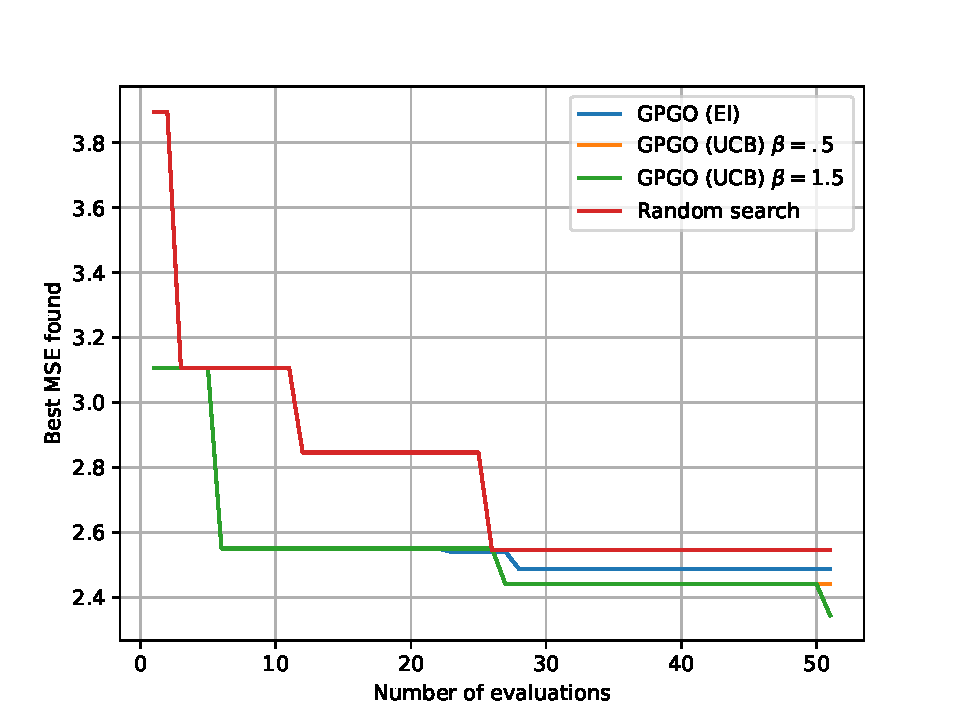
\includegraphics[scale=0.75]{figures/chapter4/aff/svm}
\label{fig:affsvm}
\end{figure}

\begin{figure}
\centering
\caption{MLP results for the binding affinity dataset.}
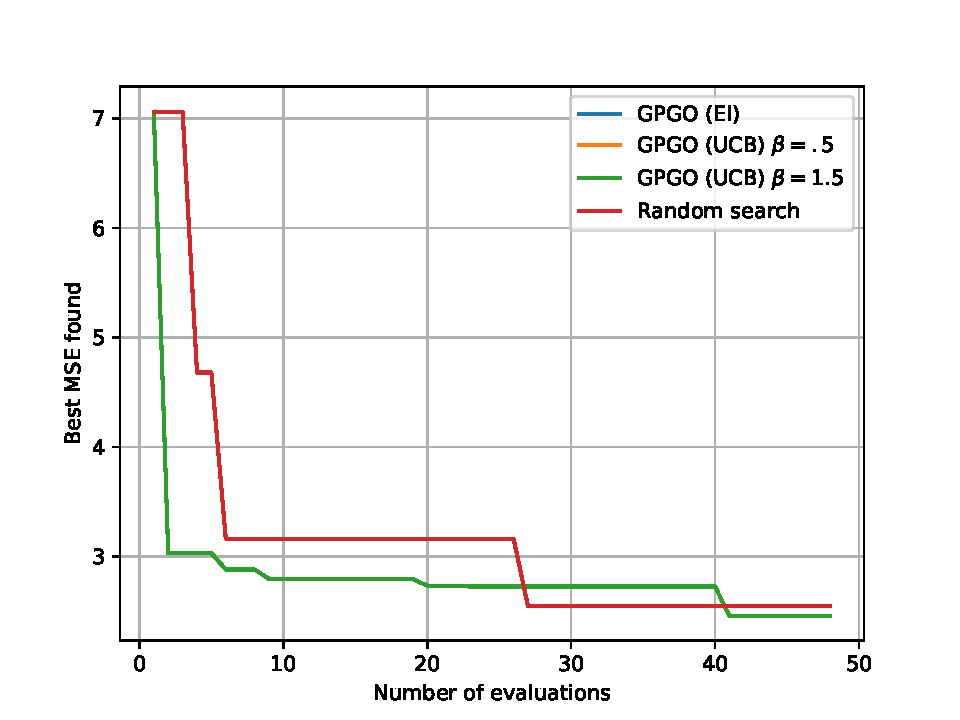
\includegraphics[scale=0.75]{figures/chapter4/aff/mlp}
\label{fig:affmlp}
\end{figure}

\begin{figure}
\centering
\caption{AdaBoost results for the binding affinity dataset.}
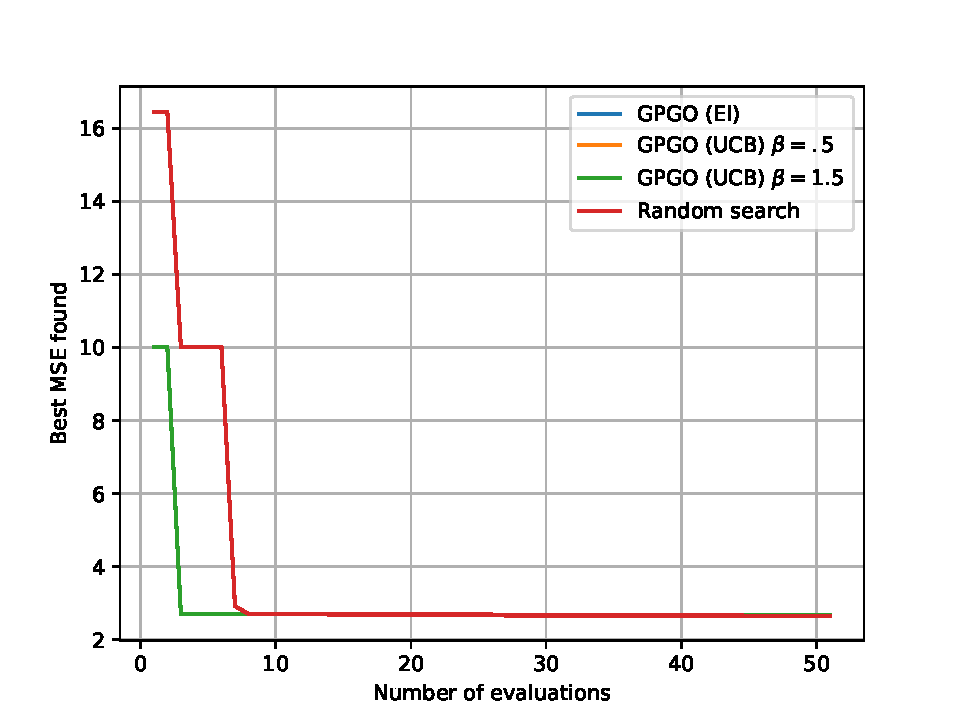
\includegraphics[scale=0.75]{figures/chapter4/aff/ada}
\label{fig:affada}
\end{figure}

\begin{figure}
\centering
\caption{Gradient Boosting Machine results for the binding affinity dataset.}
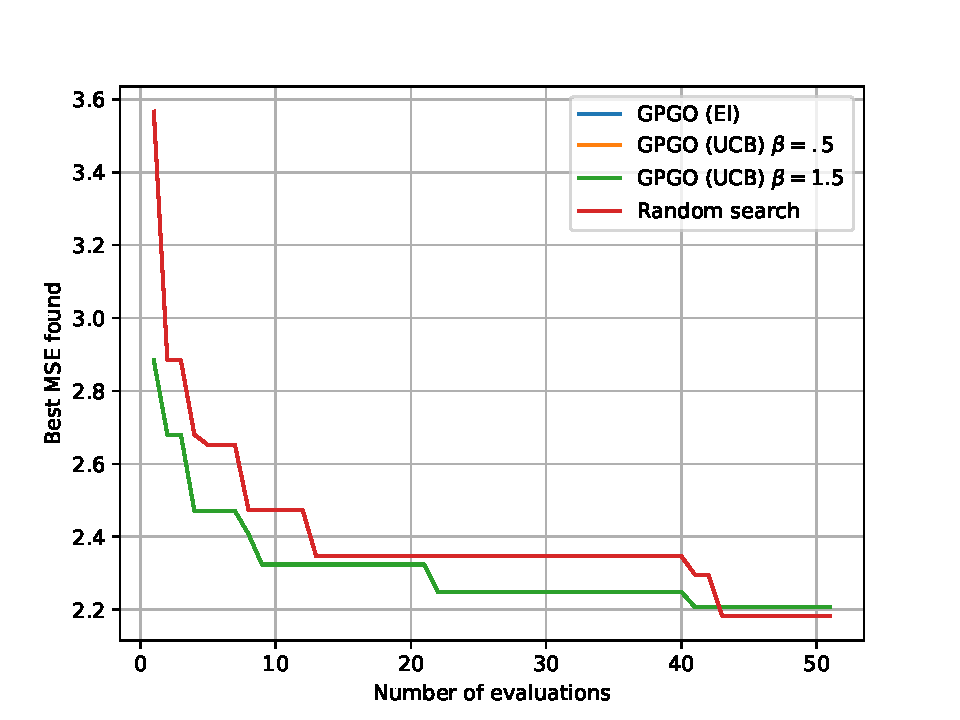
\includegraphics[scale=0.75]{figures/chapter4/aff/gbm}
\label{fig:affgbm}
\end{figure}

\newpage

\section{The protein-protein interface prediction dataset}

\chapter{pyGPGO: A simple Python Package for Bayesian Optimization}

In this chapter, we will explain the functionalities behind pyGPGO, the Bayesian Optimization software developed during this Master's thesis. pyGPGO aims to be minimalistic, modular, complete in functionality and up-to-date with latest research. pyGPGO is under the MIT License, which means it can be used for both academic and commercial purposes, while providing no warranty for the user. For more information about the MIT License, please check [ref].\\

In summary, pyGPGO is a Python package to perform Bayesian Optimization with minimal effort from the user. First we will discuss installation details, followed by a detailed description of its functionality. Then several examples of usage will be shown, which will hopefully be useful for end users or machine-learning practitioners. Later, we will compare pyGPGO to other existing Bayesian Optimization software in terms of features. In the end, future improvements on pyGPGO will be discussed.

\section{Installation}

pyGPGO comes in the form of a Python package. Only Python versions equal or higher than 3.5 are currently supported. In principle, pyGPGO should work with Windows, OSX and Linux, though only the latter has been tested. Most Unix based systems already come with Python distribution installed. To check whether it on a bash/cmd terminal:

\begin{minted}[mathescape,
               linenos,
               numbersep=5pt,
               gobble=0,
               frame=lines,
               framesep=2mm]{bash}
python --version   
\end{minted}

If Python is not installed on the system, we highly recommend installing the Python distribution Anaconda [ref]. Along with the distribution, they also provide most common packages for numeric/scientific operations. In particular, should the user choose to install the Anaconda distribution all dependencies needed by pyGPGO are covered. After downloading the executable corresponding to your particular system configuration from their web page, it suffices to do (for UNIX-based systems):

\begin{minted}[mathescape,
               linenos,
               numbersep=5pt,
               gobble=0,
               frame=lines,
               framesep=2mm]{bash}
bash Anaconda3-x.x.x-Linux-x86_64.sh
\end{minted}

Follow the instructions to install it on a local path in your system. In particular, the Anaconda installer will ask if the user wants to prepend to the system \texttt{PATH} the route to the Python binaries. Windows users have a graphical installer available in the Anaconda website.\\

If the user has a working Python environment in the system and does not want to use the one provided by Anaconda, some dependencies must be fulfilled in order for pyGPGO to work. In particular, both \texttt{numpy} and \texttt{joblib} need to be installed. Typically, one should use the packages available in the Python Package Index (PyPI) and install them using the Python Package manager \texttt{pip}. From a bash terminal:

\begin{minted}[mathescape,
               linenos,
               numbersep=5pt,
               gobble=0,
               frame=lines,
               framesep=2mm]{bash}
pip install --upgrade numpy joblib            
\end{minted}

pyGPGO is available as well in PyPI, to install the latest \textit{stable} version it suffices to execute:
 
\begin{minted}[mathescape,
               linenos,
               numbersep=5pt,
               gobble=0,
               frame=lines,
               framesep=2mm]{bash}
pip install pyGPGO           
\end{minted}

To get the bleeding-edge version of pyGPGO, one can also retrieve it from the associated GitHub repository:

\begin{minted}[mathescape,
               linenos,
               numbersep=5pt,
               gobble=0,
               frame=lines,
               framesep=2mm]{bash}
pip install git+https://github.com/hawk31/pyGPGO          
\end{minted}

\section{Usage}

pyGPGO aims to be an easy to use package to perform Bayesian Optimization. All functionality is divided in different modules, each performing a very specific task. We go briefly over the different modules here, but they will be discussed in detail in Section \ref{features}.

\begin{itemize}
\item The \texttt{covfunc} module contains all the code related to covariance function calculations. 
\item The \texttt{GPRegressor} module implements regular Gaussian Process regression.
\item The \texttt{Acquisition} module lets the user specify different acquisition function strategies.
\item The \texttt{GPGO} module implements Bayesian Optimization procedures. 
\end{itemize}

Apart from this functionality, there is plenty of material in the GitHub repository of this package:

\begin{itemize}
\item A folder named \texttt{examples}, with all the coding examples laid down throughout the course of this master's thesis.
\item A folder named \texttt{testing} with all the code used regarding benchmarking and testing of the datasets used in Chapter 4 of this work.
\item A folder named \texttt{datasets} with all the datasets tested in Chapter 4, in .csv format. 
\end{itemize}

\subsection{A minimal example}

Here we go through a minimal example to show how to use pyGPGO in its most simple form. We comment line by line using the IPython console.

\begin{minted}[mathescape,
               linenos,
               numbersep=5pt,
               gobble=0,
               frame=lines,
               framesep=2mm,
               python3=true]{python}
In [1]: import numpy as np
   ...: import matplotlib.pyplot as plt
   ...: from pyGPGO.covfunc import squaredExponential
   ...: from pyGPGO.GPRegressor import GPRegressor
   ...: from pyGPGO.acquisition import Acquisition
   ...: from pyGPGO.GPGO import GPGO               
\end{minted}

After loading \texttt{numpy} and \texttt{matplotlib}, we start loading all the needed modules for our example: we will use the \texttt{squaredExponential} covariance function, a Gaussian Process regressor \texttt{GPRegressor}, an \texttt{Acquisition} function and \texttt{GPGO}, the class for Bayesian Optimization. We fix a random seed, and define the function we are about to optimize, a plot of which is available in Figure \ref{fig:exfun}.

\begin{minted}[mathescape,
               linenos,
               numbersep=5pt,
               gobble=0,
               frame=lines,
               framesep=2mm,
               python3=true]{python}
In [2]:     np.random.seed(20)
   ...:     def f(x):
   ...:         return -((6*x-2)**2*np.sin(12*x-4))
\end{minted}

\begin{figure}
\centering
\caption{Example function for optimization with pyGPGO.}
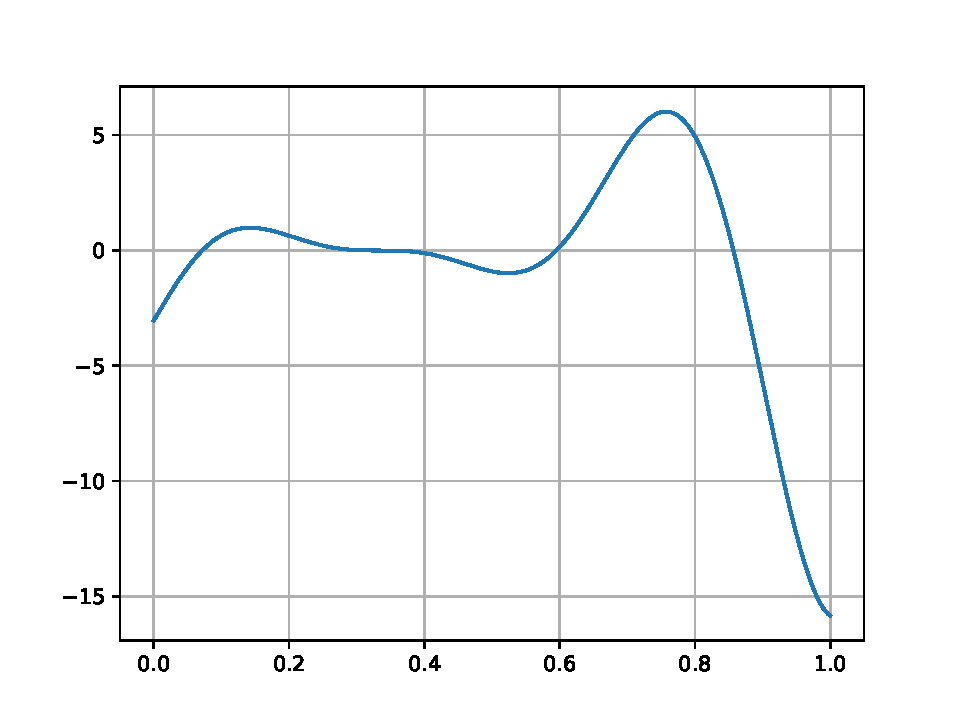
\includegraphics[width=0.75\textwidth]{figures/chapter5/exfun}
\label{fig:exfun}
\end{figure}


We now instantiate our covariance function, our regressor and our acquisition:

\begin{minted}[mathescape,
               linenos,
               numbersep=5pt,
               gobble=0,
               frame=lines,
               framesep=2mm,
               python3=true]{python}
In [3]:     sexp = squaredExponential()
   ...:     gp = GPRegressor(sexp)
   ...:     acq = Acquisition(mode = 'ExpectedImprovement')
\end{minted}

We define our the parameters to optimize over now, as a dictionary. Note that function \texttt{f} takes as parameter \texttt{x}. It is a continuous variable, where $x\in \left[0, 1\right]$. If we had other variables, we simply add them to the dictionary with its type and bounds.

\begin{minted}[mathescape,
               linenos,
               numbersep=5pt,
               gobble=0,
               frame=lines,
               framesep=2mm,
               python3=true]{python}
In [4]:     params = {'x': ('cont', (0, 1))}
\end{minted}

We now instantiate our \texttt{GPGO} class, passing all previous created objects:

\begin{minted}[mathescape,
               linenos,
               numbersep=5pt,
               gobble=0,
               frame=lines,
               framesep=2mm,
               python3=true]{python}
In [5]:	gpgo = GPGO(gp, acq, f, params)
\end{minted}

We finally optimize for a number of iterations:

\begin{minted}[mathescape,
               linenos,
               numbersep=5pt,
               gobble=0,
               frame=lines,
               framesep=2mm,
               python3=true]{python}
In [6]: gpgo.run(max_iter = 10)               
\end{minted}

Check the result just by calling:

\begin{minted}[mathescape,
               linenos,
               numbersep=5pt,
               gobble=0,
               frame=lines,
               framesep=2mm,
               python3=true]{python}
In [7]: gpgo.getResult()
Out [8]:	 (OrderedDict([('x', 0.76321944301549549)]), 6.0013872547078249)
\end{minted}

After 10 iterations, the best value for \texttt{x} our optimizer has found is $0.7632$, with a function value of $6.001$.

\section{Examples}

In this section, we will detail several examples on how to use pyGPGO for real world tasks. They will provide extra details on how much functionality the package exposes to the end user and may serve as a blueprint for other tasks.

\subsection{Gaussian Process regression using the \texttt{GPRegressor} module.}

While pyGPGO is mainly a Bayesian Optimization package, it also exposes a very competent class for performing Gaussian Process regression. While the main features of this class are discussed in Section \ref{features}, we provide a simple example on how to perform GP Regression on noisy synthetic data. The script below produces Figure \ref{fig:noiseopt}.

\begin{minted}[mathescape,
               linenos,
               numbersep=5pt,
               gobble=0,
               frame=lines,
               framesep=2mm,
               python3=true]{python}
import numpy as np
import matplotlib.pyplot as plt
from pyGPGO.GPGO import GPGO
from pyGPGO.GPRegressor import GPRegressor
from pyGPGO.acquisition import Acquisition
from pyGPGO.covfunc import squaredExponential


if __name__ == '__main__':
    rng = np.random.RandomState(0)
    X = rng.uniform(0, 5, 20)[:, np.newaxis]
    y = 0.5 * np.sin(3 * X[:, 0]) + rng.normal(0, 0.5, X.shape[0])

    sexp = squaredExponential()
    gp = GPRegressor(sexp, optimize = True, usegrads = True)
    gp.fit(X, y)

    X_ = np.linspace(0, 5, 100)
    y_mean, y_var = gp.predict(X_[:, np.newaxis], return_std=True)
    y_std = np.sqrt(y_var)
    plt.plot(X_, y_mean, 'k', lw=2, zorder=9, label = 'Posterior mean')
    plt.fill_between(X_, y_mean - 1.64 * y_std,
                     y_mean + 1.64 * y_std,
                     alpha=0.4, color='blue')
    plt.plot(X_, 0.5*np.sin(3*X_), 'r', lw=2, zorder=9, label = 'Original function')
    plt.scatter(X[:, 0], y, c='r', s=50, zorder=10)
    plt.legend(loc = 0)
    params = gp.getcovparams()
    plt.title('Optimal params | \$l\$={}, \$\sigma_n^2\$
    ={},\sigma_f^2={}'.format(np.round(params['l'],3),
    	  np.round(params['sigmaf'], 3), np.round(params['sigman'], 3)))
    plt.tight_layout()
    plt.show()
\end{minted}


A few notes on the code, notice that we add two extra parameters to the \texttt{GPRegressor} module: \texttt{optimize=True, usegrads=True} indicates to the instance that it should perform Type II maximum likelihood estimation of the \texttt{squaredExponential} instance hyper-parameters using gradient information if available. By default all hyper-parameters are optimized, in this case, $\left\lbrace l, \sigma_n^2, \sigma_f^2 \right\rbrace$ are optimized. If we want only a subset of them to be optimized or none at all, we can specify so in the corresponding covariance function instance. 



\subsection{Optimizing parameters of a machine-learning model using the \texttt{GPGO} module.}

While pyGPGO can optimize any function the user specifies, the main topic of this main thesis was the application of these algorithms to optimize the hyperparameters of machine-learning algorithms. We provide a very simple way of how to do so using \texttt{scikit-learn}, arguably the most complete machine-learning package for Python. The example generates synthetic data and tries to optimize a Support Vector Machine classifier parameters ($C, \gamma$), using cross-validation. A plot of the generated data can be checked in Figure \ref{fig:makemoons}.\\

\begin{minted}[mathescape,
               linenos,
               numbersep=5pt,
               gobble=0,
               frame=lines,
               framesep=2mm,
               python3=true]{python}
import numpy as np
import matplotlib.pyplot as plt
from matplotlib.colors import ListedColormap
from sklearn.datasets import make_moons
from sklearn.svm import SVC
from sklearn.model_selection import cross_val_score


from pyGPGO.GPGO import GPGO
from pyGPGO.GPRegressor import GPRegressor
from pyGPGO.acquisition import Acquisition
from pyGPGO.covfunc import squaredExponential


def evaluateModel(C, gamma):
    clf = SVC(C=C, gamma=gamma)
    return np.average(cross_val_score(clf, X, y))
    

if __name__ == '__main__':
    np.random.seed(20)
    X, y = make_moons(n_samples = 200, noise = 0.3)

    cm_bright = ListedColormap(['#fc4349', '#6dbcdb'])
    
    fig = plt.figure()
    plt.scatter(X[:, 0], X[:, 1], c = y, cmap = cm_bright)
    plt.show()
    
    sexp = squaredExponential()
    gp = GPRegressor(sexp, optimize = True, usegrads = True)
    acq = Acquisition(mode = 'UCB', beta = 1.5)

    params = {'C':      ('cont', (1e-4, 1e4)),
              'gamma':  ('cont', (1e-4, 10))
             }

    gpgo = GPGO(gp, acq, evaluateModel, params)
    gpgo.run(max_iter = 50)
    gpgo.getResult()               
\end{minted}

\FloatBarrier
\begin{figure}
\centering
\caption{Gaussian Process regression of noisy inputs with pyGPGO.}
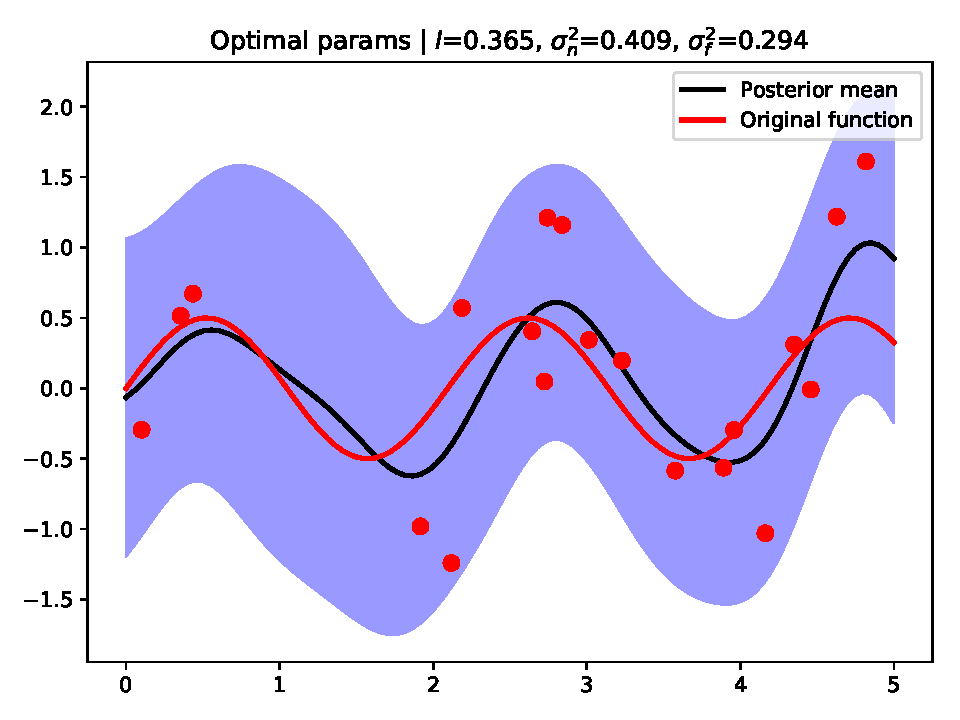
\includegraphics[width=0.75\textwidth]{figures/chapter5/noiseopt}
\label{fig:noiseopt}
\end{figure}

\begin{figure}
\centering
\caption{Synthetic data generated for our \texttt{sklearn} optimization example.}
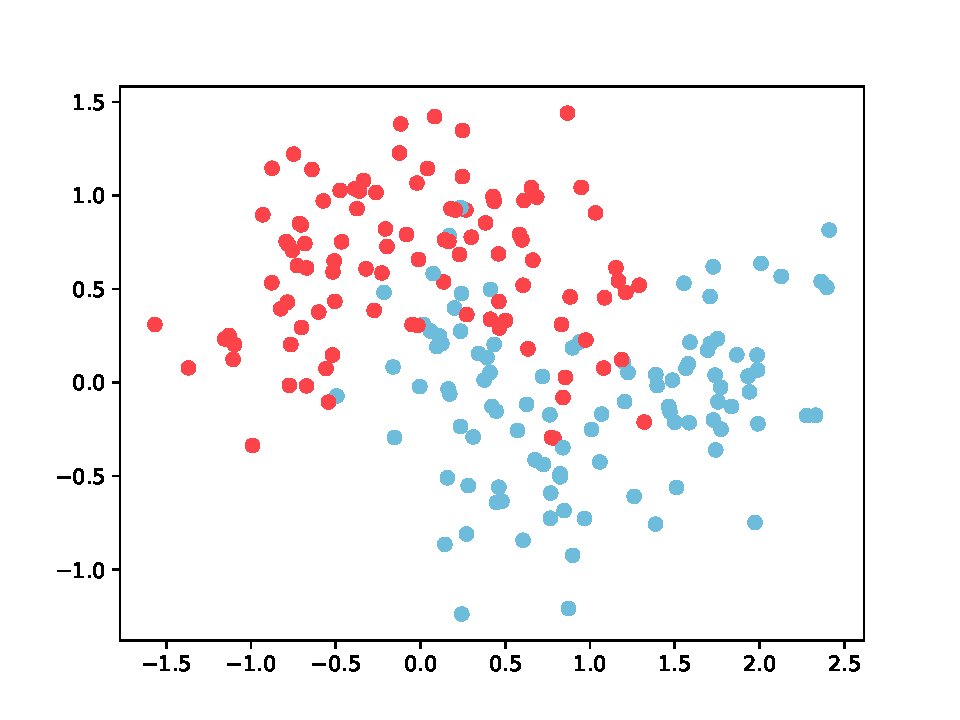
\includegraphics[width=0.75\textwidth]{figures/chapter5/makemoons}
\label{fig:makemoons}
\end{figure}




\section{Features}\label{features}
\section{Comparison with existing software}
\section{Future work}

\chapter*{Appendix}
\section*{Examples code}
\subsection*{drawGP.py}
\label{drawGP}
\begin{minted}[mathescape,
               linenos,
               numbersep=5pt,
               gobble=0,
               frame=lines,
               framesep=2mm,
               python3 = true]{python}
import numpy as np
from numpy.random import multivariate_normal
from covfunc import squaredExponential
import matplotlib.pyplot as plt

if __name__ == '__main__':
        np.random.seed(93)
        # Equally spaced values of Xstar
        Xstar = np.arange(0, 2 * np.pi, step = np.pi/16)
        Xstar = np.array([np.atleast_2d(x) for x in Xstar])[:, 0]
        sexp = squaredExponential()
        # By default assume mean 0
        m = np.zeros(Xstar.shape[0])
        # Compute squared-exponential matrix
        K = sexp.K(Xstar, Xstar)

        n_samples = 3
        # Draw samples from multivariate normal
        samples = multivariate_normal(m, K, size = n_samples)

        # Plot values
        x = Xstar.flatten()
        plt.figure()
        for i in range(n_samples):
                plt.plot(x, samples[i], label = 'GP sample {}'.format(i + 1))
        plt.xlabel('x')
        plt.ylabel('y')
        plt.title('Sampled GP priors from Squared Exponential kernel')
        plt.grid()
        plt.legend(loc = 0)
        plt.show()	
\end{minted}

\subsection*{sineGP.py}
\label{sineGP}
\begin{minted}[mathescape,
               linenos,
               numbersep=5pt,
               gobble=0,
               frame=lines,
               framesep=2mm,
               python3 = true]{python}
import numpy as np
from GPRegressor import GPRegressor
from covfunc import squaredExponential
import matplotlib.pyplot as plt

if __name__ == '__main__':
    # Build synthetic data (sine function)
    x = np.arange(0, 2 * np.pi + 0.01, step=np.pi / 2)
    y = np.sin(x)
    X = np.array([np.atleast_2d(u) for u in x])[:, 0]

    # Specify covariance function
    sexp = squaredExponential()
    # Instantiate GPRegressor class
    gp = GPRegressor(sexp)
    # Fit the model to the data
    gp.fit(X, y)

    # Predict on new data
    xstar = np.arange(0, 2 * np.pi, step=0.01)
    Xstar = np.array([np.atleast_2d(u) for u in xstar])[:, 0]
    ymean, ystd = gp.predict(Xstar, return_std=True)

    # Confidence interval bounds
    lower, upper = ymean - 1.96 * ystd, ymean + 1.96 * ystd

    # Plot values
    plt.figure()
    plt.plot(xstar, ymean, label='Posterior mean')
    plt.plot(xstar, np.sin(xstar), label='True function')
    plt.fill_between(xstar, lower, upper, alpha=0.4, label='95% confidence band')
    plt.grid()
    plt.legend(loc=0)
    plt.show()
   \end{minted}
   \subsection*{covzoo.py}
   \label{covzoo}
   \begin{minted}[mathescape,
               linenos,
               numbersep=5pt,
               gobble=0,
               frame=lines,
               framesep=2mm,
               python3 = true]{python}
import numpy as np
from covfunc import *
from GPRegressor import GPRegressor
import matplotlib.pyplot as plt


if __name__ == '__main__':
        # Build synthetic data (sine function)
        x = np.arange(0, 2 * np.pi + 0.01, step = np.pi / 2)
        y = np.sin(x)
        X = np.array([np.atleast_2d(u) for u in x])[:, 0]

        # Covariance functions to loop over
        covfuncs = [squaredExponential(), matern(), gammaExponential(), rationalQuadratic()]
        titles = [r'Squared Exponential ($l = 1$)', r'Matern ($\nu = 1$, $l = 1$)',
         r'Gamma Exponential ($\gamma = 1, l = 1$)', r'Rational Quadratic ($\alpha = 1, l = 1$)']
        plt.figure()
        plt.rc('text', usetex=True)
        for i, cov in enumerate(covfuncs):
                gp = GPRegressor(cov)
                gp.fit(X, y)
                xstar = np.arange(0, 2 * np.pi, step = 0.01)
                Xstar = np.array([np.atleast_2d(u) for u in xstar])[:, 0]
                ymean, ystd = gp.predict(Xstar, return_std = True)
                
                lower, upper = ymean - 1.96 * ystd, ymean + 1.96 * ystd
                plt.subplot(2, 2, i + 1)
                plt.plot(xstar, ymean, label = 'Posterior mean')
                plt.plot(xstar, np.sin(xstar), label = 'True function')
                plt.fill_between(xstar, lower, upper, alpha = 0.4,
                 label = '95\% confidence band')
                plt.grid()
                plt.title(titles[i])
        plt.legend(loc = 0)
        plt.show()
\end{minted}

\subsection*{hyperopt.py}
\label{hyperopt}
\begin{minted}[mathescape,
               linenos,
               numbersep=5pt,
               gobble=0,
               frame=lines,
               framesep=2mm,
               python3 = true]{python}
import numpy as np
from GPRegressor import GPRegressor
from covfunc import squaredExponential
import matplotlib.pyplot as plt

def gradient(gp, sexp):
        alpha = gp.alpha
        K = gp.K
        gradK = sexp.gradK(gp.X, gp.X, 'l')
        inner = np.dot(np.atleast_2d(alpha).T, np.atleast_2d(alpha)) - np.linalg.inv(K)
        return(.5 * np.trace(np.dot(inner, gradK)))


if __name__ == '__main__':
        x = np.arange(0, 2 * np.pi + 0.01, step = np.pi / 2)
        X = np.array([np.atleast_2d(u) for u in x])[:, 0]
        y = np.sin(x)

        logp = []
        grad = []
        length_scales = np.linspace(0.1, 2, 1000)

        for l in length_scales:
                sexp = squaredExponential(l = l)
                gp = GPRegressor(sexp)
                gp.fit(X, y)
                logp.append(gp.logp)
                grad.append(gradient(gp, sexp))

        plt.figure()
        plt.subplot(2, 1, 1)
        plt.plot(length_scales, logp)
        plt.title('Marginal log-likelihood')
        plt.xlabel('Characteristic length-scale l')
        plt.ylabel('log-likelihood')
        plt.grid()
        plt.subplot(2, 1, 2)
        plt.plot(length_scales, grad, '--', color = 'red')
        plt.title('Gradient w.r.t. l')
        plt.xlabel('Characteristic length-scale l')
        plt.grid()
        plt.show()
\end{minted}

\subsection*{acqzoo.py}


\begin{minted}[mathescape,
               linenos,
               numbersep=5pt,
               gobble=0,
               frame=lines,
               framesep=2mm,
               python3 = true]{python}
import numpy as np
from GPRegressor import GPRegressor
from acquisition import Acquisition
from covfunc import squaredExponential
from GPGO import GPGO


def plotGPGO(gpgo, param, index, new = True):
        param_value = list(param.values())[0][1]
        x_test = np.linspace(param_value[0], param_value[1], 1000).reshape((1000, 1))
        y_hat, y_var = gpgo.GP.predict(x_test, return_std = True)
        std = np.sqrt(y_var)
        l, u = y_hat - 1.96 * std, y_hat + 1.96 * std
        if new:
                plt.figure()
                plt.subplot(5, 1, 1)
                plt.fill_between(x_test.flatten(), l, u, alpha = 0.2)
                plt.plot(x_test.flatten(), y_hat)
        plt.subplot(5, 1, index)
        a = np.array([-gpgo._acqWrapper(np.atleast_1d(x)) for x in x_test]).flatten()
        plt.plot(x_test, a, color = colors[index - 2], label = acq_titles[index - 2])
        gpgo._optimizeAcq(method = 'L-BFGS-B', n_start = 1000)
        plt.axvline(x = gpgo.best)
        plt.legend(loc = 0)
        


if __name__ == '__main__':
        def f(x):
                return(np.sin(x))

        acq_1 = Acquisition(mode = 'ExpectedImprovement')
        acq_2 = Acquisition(mode = 'ProbabilityImprovement')
        acq_3 = Acquisition(mode = 'UCB', beta = 0.5)
        acq_4 = Acquisition(mode = 'UCB', beta = 1.5)
        acq_list = [acq_1, acq_2, acq_3, acq_4]
        sexp = squaredExponential()
        param = {'x': ('cont', [0, 2 * np.pi])}
        new = True
        colors = ['green', 'red', 'orange', 'black']
        acq_titles = [r'Expected improvement', r'Probability of Improvement',
         r'GP-UCB $\beta = .5$', r'GP-UCB $\beta = 1.5$']

        for index, acq in enumerate(acq_list):
                np.random.seed(200)
                gp = GPRegressor(sexp)
                gpgo = GPGO(gp, acq, f, param)
                gpgo._firstRun(n_eval = 3)
                plotGPGO(gpgo, param, index = index + 2, new = new)
                new = False

        plt.show()                  
\end{minted}

\subsection*{bayoptwork.py}
\label{bayoptwork}

\begin{minted}[mathescape,
               linenos,
               numbersep=5pt,
               gobble=0,
               frame=lines,
               framesep=2mm,
               python3 = true]{python}

import numpy as np
from GPRegressor import GPRegressor
from covfunc import squaredExponential
import matplotlib.pyplot as plt

if __name__ == '__main__':
    # Build synthetic data (sine function)
    x = np.arange(0, 2 * np.pi + 0.01, step=np.pi / 1.5)
    y = np.sin(x)
    X = np.array([np.atleast_2d(u) for u in x])[:, 0]

    # Specify covariance function
    sexp = squaredExponential()
    # Instantiate GPRegressor class
    gp = GPRegressor(sexp)
    # Fit the model to the data
    gp.fit(X, y)

    # Predict on new data
    xstar = np.arange(0, 2 * np.pi, step=0.01)
    Xstar = np.array([np.atleast_2d(u) for u in xstar])[:, 0]
    ymean, ystd = gp.predict(Xstar, return_std=True)

    # Confidence interval bounds
    lower, upper = ymean - 1.96 * ystd, ymean + 1.96 * ystd

    # Plot values
    plt.figure()
    plt.plot(xstar, ymean, label='Posterior mean')
    plt.plot(xstar, lower, '--', label='Lower confidence bound')
    plt.plot(xstar, upper, '--', label='Upper confidence bound')
    plt.axhline(y=np.max(lower), color='black')
    plt.axvspan(0, .68, color='grey', alpha=0.3)
    plt.plot(xstar[np.argmax(lower)], np.max(lower), '*', markersize=20)
    plt.axvspan(3.04, 7, color='grey', alpha=0.3, label='Discarded region')
    plt.text(3.75, 0.75, 'max LCB')
    plt.grid()
    plt.legend(loc=0)
    plt.show()                      
\end{minted}

\subsection*{sineopt.py}
\label{sineopt}

\begin{minted}[mathescape,
               linenos,
               numbersep=5pt,
               gobble=0,
               frame=lines,
               framesep=2mm,
               python3 = true]{python}

import os

import matplotlib.pyplot as plt

from GPGO import GPGO
from GPRegressor import GPRegressor
from acquisition import Acquisition
from covfunc import *


def plotGPGO(gpgo, param):
    param_value = list(param.values())[0][1]
    x_test = np.linspace(param_value[0], param_value[1], 1000).reshape((1000, 1))
    hat = gpgo.GP.predict(x_test, return_std=True)
    y_hat, y_std = hat[0], np.sqrt(hat[1])
    l, u = y_hat - 1.96 * y_std, y_hat + 1.96 * y_std
    fig = plt.figure()
    r = fig.add_subplot(2, 1, 1)
    r.set_title('Fitted Gaussian process')
    plt.fill_between(x_test.flatten(), l, u, alpha=0.2)
    plt.plot(x_test.flatten(), y_hat, color='red', label='Posterior mean')
    plt.legend(loc=0)
    a = np.array([-gpgo._acqWrapper(np.atleast_1d(x)) for x in x_test]).flatten()
    r = fig.add_subplot(2, 1, 2)
    r.set_title('Acquisition function')
    plt.plot(x_test, a, color='green')
    gpgo._optimizeAcq(method='L-BFGS-B', n_start=1000)
    plt.axvline(x=gpgo.best, color='black', label='Found optima')
    plt.legend(loc=0)
    plt.tight_layout()
    plt.savefig(os.path.join(os.getcwd(), 'mthesis_text/figures/chapter3/sine/{}.pdf'.format(i)))
    plt.show()


if __name__ == '__main__':
    np.random.seed(321)


    def f(x):
        return (np.sin(x))


    sexp = squaredExponential()
    gp = GPRegressor(sexp)
    acq = Acquisition(mode='ExpectedImprovement')
    param = {'x': ('cont', [0, 2 * np.pi])}

    gpgo = GPGO(gp, acq, f, param, n_jobs=-1)
    gpgo._firstRun()

    for i in range(6):
        plotGPGO(gpgo, param)
        gpgo.updateGP()

\end{minted}

\subsection*{rastriginopt.py}
\label{rastriginopt}

\begin{minted}[mathescape,
               linenos,
               numbersep=5pt,
               gobble=0,
               frame=lines,
               framesep=2mm,
               python3 = true]{python}
               
import os
from collections import OrderedDict

import matplotlib.pyplot as plt

from GPGO import GPGO
from GPRegressor import GPRegressor
from acquisition import Acquisition
from covfunc import *


def rastrigin(x, y, A=10):
    return (2 * A + (x ** 2 - A * np.cos(2 * np.pi * x)) + (y ** 2 - A * np.cos(2 * np.pi * y)))


def plot_f(x_values, y_values, f):
    z = np.zeros((len(x_values), len(y_values)))
    for i in range(len(x_values)):
        for j in range(len(y_values)):
            z[i, j] = f(x_values[i], y_values[j])
    plt.imshow(z.T, origin='lower', extent=[np.min(x_values), np.max(x_values), np.min(y_values), np.max(y_values)])
    plt.colorbar()
    plt.show()
    plt.savefig(os.path.join(os.getcwd(), 'mthesis_text/figures/chapter3/rosen/rosen.pdf'))


def plot2dgpgo(gpgo):
    tested_X = gpgo.GP.X
    n = 100
    r_x, r_y = gpgo.parameter_range[0], gpgo.parameter_range[1]
    x_test = np.linspace(r_x[0], r_x[1], n)
    y_test = np.linspace(r_y[0], r_y[1], n)
    z_hat = np.empty((len(x_test), len(y_test)))
    z_var = np.empty((len(x_test), len(y_test)))
    ac = np.empty((len(x_test), len(y_test)))
    for i in range(len(x_test)):
        for j in range(len(y_test)):
            res = gpgo.GP.predict([x_test[i], y_test[j]])
            z_hat[i, j] = res[0]
            z_var[i, j] = res[1][0]
            ac[i, j] = -gpgo._acqWrapper(np.atleast_1d([x_test[i], y_test[j]]))
    fig = plt.figure()
    a = fig.add_subplot(2, 2, 1)
    a.set_title('Posterior mean')
    plt.imshow(z_hat.T, origin='lower', extent=[r_x[0], r_x[1], r_y[0], r_y[1]])
    plt.colorbar()
    plt.plot(tested_X[:, 0], tested_X[:, 1], 'wx', markersize=10)
    a = fig.add_subplot(2, 2, 2)
    a.set_title('Posterior variance')
    plt.imshow(z_var.T, origin='lower', extent=[r_x[0], r_x[1], r_y[0], r_y[1]])
    plt.plot(tested_X[:, 0], tested_X[:, 1], 'wx', markersize=10)
    plt.colorbar()
    a = fig.add_subplot(2, 2, 3)
    a.set_title('Acquisition function')
    plt.imshow(ac.T, origin='lower', extent=[r_x[0], r_x[1], r_y[0], r_y[1]])
    plt.colorbar()
    gpgo._optimizeAcq(method='L-BFGS-B', n_start=500)
    plt.plot(gpgo.best[0], gpgo.best[1], 'gx', markersize=15)
    plt.tight_layout()
    plt.savefig(os.path.join(os.getcwd(), 'mthesis_text/figures/chapter3/rosen/{}.pdf'.format(item)))
    plt.show()


if __name__ == '__main__':
    x = np.linspace(-1, 1, 1000)
    y = np.linspace(-1, 1, 1000)
    plot_f(x, y, rastrigin)

    np.random.seed(20)
    sexp = squaredExponential()
    gp = GPRegressor(sexp)
    acq = Acquisition(mode='ExpectedImprovement')

    param = OrderedDict()
    param['x'] = ('cont', [-1, 1])
    param['y'] = ('cont', [-1, 1])

    gpgo = GPGO(gp, acq, rastrigin, param, n_jobs=-1)
    gpgo._firstRun()

    for item in range(7):
        plot2dgpgo(gpgo)
        gpgo.updateGP()
               
\end{minted}

\section*{Testing code}

\end{document}